% !TeX encoding = UTF-8
\documentclass[twoside,english,1p,final,sort&compress]{elsarticle}
\usepackage[T1]{fontenc}
\usepackage[utf8]{inputenc}
\pagestyle{headings}
\usepackage{amsthm}
\usepackage{gensymb}
\usepackage{xspace}
\usepackage{amsmath}
\usepackage{accents}
\usepackage{multirow}
\usepackage{arydshln}
\usepackage{xcolor}
\usepackage{amssymb}
\usepackage{subcaption}
\usepackage{adjustbox}
\usepackage{placeins}
\usepackage[colorlinks = true]{hyperref}

% To have Times only in text not maths
\renewcommand{\rmdefault}{ptm}

\makeatletter

\theoremstyle{plain}
\newtheorem{thm}{\protect\theoremname}

% specify here the journal
\journal{International Journal of Mechanical Sciences}

% use this if you need line numbers
\usepackage{lineno}

\makeatother

\usepackage{babel}
\providecommand{\theoremname}{Theorem}

\newcommand{\w}{\mbox{\large\ensuremath{\mathsf{w}}}}
\newcommand{\dotp}{\boldsymbol{\cdot}}
%\newcommand{\ccirc}{\kern0.5ex\vcenter{\hbox{$\scriptstyle\circ$}}\kern0.5ex}
%\newcommand{\e}[1]{\exp\left({#1}\right)}
\newcommand{\e}[1]{{\rm e}^{#1}}
\newcommand{\lay}[1]{^{(#1)}}
\newcommand{\mdot}[1]{\accentset{\mbox{\bfseries .}}{#1}}
\newcommand*{\ie}{\emph{i.e.}\@\xspace}
\newcommand*{\versus}{\emph{vs.}\@\xspace}
\newcommand*{\eal}{et \emph{al.}\@\xspace}
\newcommand*{\eg}{e.g.,\@\xspace}
\newcommand{\RMSE}{\text{E}_\text{RMS}}
\newcommand{\AARE}{\text{E}_\text{AAR}}
\newcommand{\R}{\text{R}}
\newcommand{\ps}{\text{s}^{-1}}
\DeclareMathOperator{\ANN2}{sig}
%\newcommand{\Dev}	{\mbox{\Large\ensuremath{\mathsf{s}}}}
%\DeclareMathOperator{\sech}{sech}
%\DeclareMathOperator{\ANN2}{sig}

\usepackage{esvect}
% Redefine the esvector shape to remove overlapping
\def\traitfill@#1#2#3#4{%
  $\m@th\mkern2mu\relax#4#1\mkern-1.5mu %on met \relbaredd au d\'ebut
   \cleaders\hbox{$#4\mkern-0.3mu#2\mkern-0.3mu$}\hfill %remplit avec relbareda
   \mkern-1.5mu#3$%
}
\renewcommand{\overrightarrow}{\vv}

% This is used to add comments into the text
\usepackage{soul} %Can also be used to highlight text with \hl{highlighted text}
\usepackage{color}
\definecolor{VWyellow}{RGB}{255,251,150} % VaporWave color palette
\DeclareRobustCommand{\OP}[1]{ {\begingroup\sethlcolor{VWyellow}\textcolor{red}{\hl{\textbf{Olivier Pantal\'e:} #1}}\endgroup} }

\begin{document}
\begin{frontmatter}

\title{Compararison of analytical and artificial neural network models in predicting hot deformation behavior of AISI P20 and  interpolation-extrapolation capacity validation}

\author[LGP]{Pierre Tize Mha}
\author[ETS]{Prashant Dhondapure}
\author[LGP]{Amèvi Tongne}
\author[ETS]{Mohammad Jahazi}
\author[LGP]{Olivier Pantalé \corref{cor1}}
\ead{Olivier.Pantale@enit.fr}
\ead[url]{http://www.enit.fr}

\cortext[cor1]{Corresponding author}

\address[LGP]{Laboratoire Génie de Production, INP/ENIT, Université de Toulouse, 47 Av d'Azereix, Tarbes, France 65016}
\address[ETS]{École de Technologie Supérieure, 1100 Rue Notre Dame O, Montréal, QC H3C 1K3}

\begin{abstract}
The high-temperature deformation behavior of the AISI P20 alloy was investigated by performing hot compression tests over a wide range of strains ($0.025 - 0.7$),  strain rates ($0.001\ \ps - 5\ \ps$) and temperatures ($1050\celsius-1250\celsius$).
Based on the experimental data (stress-strain curves), empirical models as the Johnson-Cook (JC), Modified-Zerilli-Armstrong (MZA), Hansel-Spittel (HS), Arhenius (AR) and PTM on the one hand and an ANN model on the other hand were developed to predict the flow behavior of this alloy.
Then, a comparative study between the analytical models and the ANN model was carried out on the basis of the calculation of some coefficients allowing to test the efficiency of each model.
These coefficients are the correlation coefficient $R$, the Average Absolute  Relative Error $\AARE$ and the Root Mean Square Error ($\RMSE$).
From these parameters it was found that the JC, MZA and HS models are not suitable for predicting the behavior of AISI P20 alloy whereas the AR and PTM models can be used for most strain rates to predict the flow behavior of this alloy.
For the strain rate ($\mdot\varepsilon = 0.01\ \ps$)  the AR model fails to describe the flow for temperatures $1050\celsius$ and $1100\celsius$  while in the case of the PTM model, the strain rate  ($\mdot\varepsilon = 0.1\ \ps$) is not well described.
This is due to the fact that this model is a sequence of polynomials which can create oscillations if the degree is high.
Regarding the ANN model, the architecture retained is composed of two hidden layers of which the first hidden layer contains $15$ neurons and the second contains $7$ neurons and the input layer contains $3$ neurons corresponding to the strain ($\varepsilon^p$), strain rate ($\mdot\varepsilon$) and temperature ($T$) and the output layer contains a single neuron corresponding to the flow stress ($\sigma^y$).
The results of the ANN model show a very good agreement between the predictions and the experiment.
This demonstrates that this  formulation of constitutive law exceeds highly the analytical models in terms of prediction.
To validate the performance of these models their capacities to interpolate and extrapolate the data were also tested where all the models relatively prove a good interpolation capacity whereas this is not the case for extrapolation where only the AR, PTM and ANN models are acceptable but still mentioning that the ANN model remains the best in both interpolation and extrapolation.
\end{abstract}

\begin{keyword}
Zerilli-Armstrong flow law \sep Constitutive behavior \sep Arhenius flow law \sep Hansel-Spittel flow law \sep Johnson-Cook flow law \sep interpolation \sep extrapolation \sep Artificial neural network
\end{keyword}

\end{frontmatter}
\linenumbers

%--------------------------------------------------------------------------
\section{Introduction\label{sec:Introduction}}
%--------------------------------------------------------------------------
Continuous casting and rolling techniques are an integral part of material forming methods.
Advantages of this method include increased process efficiency, energy savings, improved casting quality and easier mechanization and automation.
Deformation, a complex process involving simultaneous elastic and plastic deformation, is accompanied by high temperatures, high strain rates, and complex and variable frictional conditions \cite{He-2013}, for which, analytical methods are not available for quantitative study and analysis of the deformation mechanism.
On the other hand, conducting experimental tests is not only time-consuming but also requires a high financial investment \cite{Changizian-2012}.
As an alternative approach to the previous two, the Finite Element Method (FEM) is widely used as a tool for analysis and optimization of process parameters in the processing of various materials.
Finite element modeling effectively compensates for the shortcomings of analytical and experimental methods and is playing an increasingly important role in determining process parameters, improving product quality, and gaining in-depth knowledge of deformation mechanisms.
For example, FEM has been widely used to simulate and analyze hot forming processes of steel, such as forging, rolling, extrusion and casting, but the quality of the numerical solution provided by this method is highly dependent on the constitutive equation of the modeled material \cite{Qin-2010, Mandal-2009, Ji-2018}.

Hot forming processes are an essential step in the manufacture of mechanical components and directly affect the final quality of the products through their strong influence on the micro-structure and mechanical properties \cite{Ashtiani-2012}.
Several metallurgical phenomena such as work hardening and dynamic softening (dynamic recovery and re-crystallization), which very often occur during hot working, influence the behavior and deformation of materials.
The complexity of the thermomechanical behavior usually leads to the fact that it can only be taken into account accurately by using a numerical approach to obtain the response of the material under the specified loading conditions.
To this end, a mathematical formulation is typically used to represent the flow of a material in a form that can be used in finite element software \cite{Lin-2008-P, Wu-2012}.

For several years, many researchers have developed methods to predict the thermomechanical behavior of materials under hot working conditions using constitutive models.
Thus, various forms of constitutive equations have been proposed to describe the flow of materials, among which, phenomenological, semi-empirical, physical models or models based on Artificial Neural Networks (ANN) \cite{Lin-2011, Shin-2010, Rusinek-2010, Pantale-2021}.
Among the large number of models available in the literature, the Johnson-Cook (JC) \cite{Johnson-1983} and Zerilli-Armstrong (ZA) \cite{Zerilli-1987} models are the best known and most widely available in finite element codes.
The Johnson-Cook model is the most widely used because it is simple to identify and use and has few parameters to determine \cite{Khan-2004, NematNasser-2003}.
However, this model, in its original state, has some shortcomings related to nonlinear coupling phenomena not taken into account in the material behavior.
We refer here to strain hardening, strain rate hardening and thermal effects that are taken into account in a non-coupled manner in the JC model as analyzed by Jia \eal \cite{Jia-2021}.
To circumvent these shortcomings, several modified forms of the Johnson-Cook model have been developed in the past \cite{Rule-1998, Vural-2003, Lin-2010, Lin-2012, Li-2013, Zhou-2019, Zhang-2015}.
Due to its more physics-based formulation, the ZA model is often preferred to the JC model because it allows the coupling of strain rate and temperature effects \cite{Johnson-1988, Voyiadjis-2005, Dey-2007}.
However, this model has other drawbacks related to the limit value of the test temperature.
Indeed, this model applies only to low strain rates and for temperatures limited to about 60~\% of $T_m$ (where $T_m$ is the melting temperature of the material) \cite{Chiou-2005, Lee-2005, Chen-2007, Lee-2006}.
Moreover, this model, in its original form, does not take into account the coupling between deformation and temperature effects \cite{Samantaray-2009}.
In order to reduce these shortcomings (and to apply this model to a wider range of temperatures) of the ZA model, modified forms of Zerilli-Armstrong (MZA) have been proposed by several authors in recent years \cite{NematNasser-2004, Lennon-2004, Muralli-2017, Cheng-2021, Muralli-2021}.

The Arrhenius-type hyperbolic sine constitutive model is one of the most widely used phenomenological models both for the prediction of the hot deformation behavior of materials and for the analysis of the micro-structure of the material under study because this model allows the estimation of the deformation energy of the material \cite{Jonas-1969, Zhang-2012, Mostafaei-2012}.
Its original formulation has been revised several times to correctly describe the resulting experimental behavior.
In order to increase the accuracy of the model, the effects of strain \cite{Slooff-2007, Li-2012, Xu-2013}, strain rate \cite{Lin-2008-C, Mandal-2009} have been considered by several authors.
For example, Sloof \eal \cite{Slooff-2007} introduced a strain-dependent parameter into the initial formulation of the Arhenius model so that his model could predict the high-temperature flow of a magnesium alloy.
Lin \eal \cite{Lin-2008-C}, on the other hand, modified the model by introducing a strain rate compensation factor.

Users of the Forge software make extensive use of the model developed by Hansel and Spittel \cite{Hensel-1978}, commonly referred to as the HS model, which is a thermo-visco-plastic model whose formulation is based on a product of functions dependent on the three physical variables.
Unlike the JC model, this formulation is based on parameters that are determined simultaneously.
This model is simple to use and has $8$ parameters that are easy to determine.
The limitation of this model is its loss of accuracy in some cases when the $8$ parameters are defined.
This is why many works often limit its identification to only $5$ or $6$ parameters.
This has been verified in our study where the smallest error of the model is obtained with only $5$ parameters identified.

The fixed and limited number of parameters imposed by each analytical model as presented above has both advantages and disadvantages.
These models have few parameters and are therefore easy to identify, but when these models have to be applied to a material different from the one for which they were initially developed they lose their performance as in the case of the HS model.
To try to solve this problem, Tize Mha \eal \cite{TizeMha-2022} has proposed a formulation where the number of parameters is not known in advance.
The idea is to make the formulation of an analytical model flexible so that it can be adapted to many materials.
This formulation is based on the MZA model and polynomial functions of undefined order are used in the identification phase.

Behavior modeling based on an artificial neural network is an approach to predict the flow of materials without requiring a mathematical formulation of the flow law.
It is therefore not necessary to postulate a mathematical expression to identify the parameters of the model.
Since the behavior of materials is highly nonlinear at high temperatures, and depends on many factors that are also nonlinear, the evaluation of the flow stress by an analytical model whose parameters are identified by a classical regression method is limited.
Faced with these limitations, ANN models are of major interest because they are particularly suited to deal with complex and nonlinear relationships.
Consequently, ANNs have been successfully applied to predict the flow of materials under hot working conditions \cite{Lin-2008-ANN, Lu-2011-ANN, Ashtiani-2016-CSP, Stoffel-2019-NNB, Pantale-2021}.
They provide a fundamentally different approach to statistical or numerical techniques for modeling materials.

In this work, the high-temperature thermomechanical behavior of AISI P20 modified carbon steel subjected to compression tests in a Gleeble thermomechanical simulator was studied.
From the experimental data obtained from the compression tests, five analytical models were identified in order to select the one that best describes the behavior of this alloy.
A flow model based on an artificial neural network was also developed and identified, and a comparative study between the five analytical models and the ANN model is proposed.
A fundamental concern addressed in this work is the ability of a model to interpolate and extrapolate the results of the model with respect to the range of conditions covered by the experimental tests.

The main parts of this work are as follows: Section \ref{sec:Materials} presents the hardware (Gleeble thermomechanical simulator), the experimental procedure, the material and the results of the compression tests performed for this study.
Section \ref{sec:ConstLaws} is devoted to the presentation of the five analytical models, the ANN model, the identification of their parameters and the comparison of the performances of these models.
Section \ref{sec:inExtrapolation} details the interpolation and extrapolation capabilities of each model proposed in this paper.
Conclusions and future work are detailed in Section \ref{sec:Conclusion}.

%----------------------------------------------
\section{Materials and Experiments\label{sec:Materials}}
%----------------------------------------------

%----------------------------------------------
\subsection{Experimental procedure}
%----------------------------------------------

The material used in this study is the modified carbon alloy AISI P20 whose chemical composition is given in Table \ref{tab:Composition}.
Cylindrical samples were machined with an initial diameter of $10$~mm and a height of $15$~mm.
A batch of $30$ hot compression tests were performed on a Gleeble-3800 thermomechanical simulator (see Figure \ref{fig:Gleeble3800}), for the five temperature levels of $1050\celsius$, $1100\celsius$, $1150\celsius$, $1200\celsius$ and $1250\celsius$ with the six strain rates of $0.001~\ps$, $0.01~\ps$, $0.1~\ps$, $1.0~\ps$, $2.0~\ps$ and $5.0~\ps$.

\begin{table}[h!]
\centering
\caption{Chemical composition of AISI P20 steel, Fe = balance.}
\begin{tabular}{lccccccc}
\hline
Element & C & Mn & Mo & Si & Ni & Cr & Cu\\ \hline
Wt~\% & 0.30 & 0.89 & 0.52 & 0.34 & 0.68 & 1.86 & 0.17\\ \hline
\label{tab:Composition}
\end{tabular}
\end{table}
\begin{figure}[!ht]
\centering
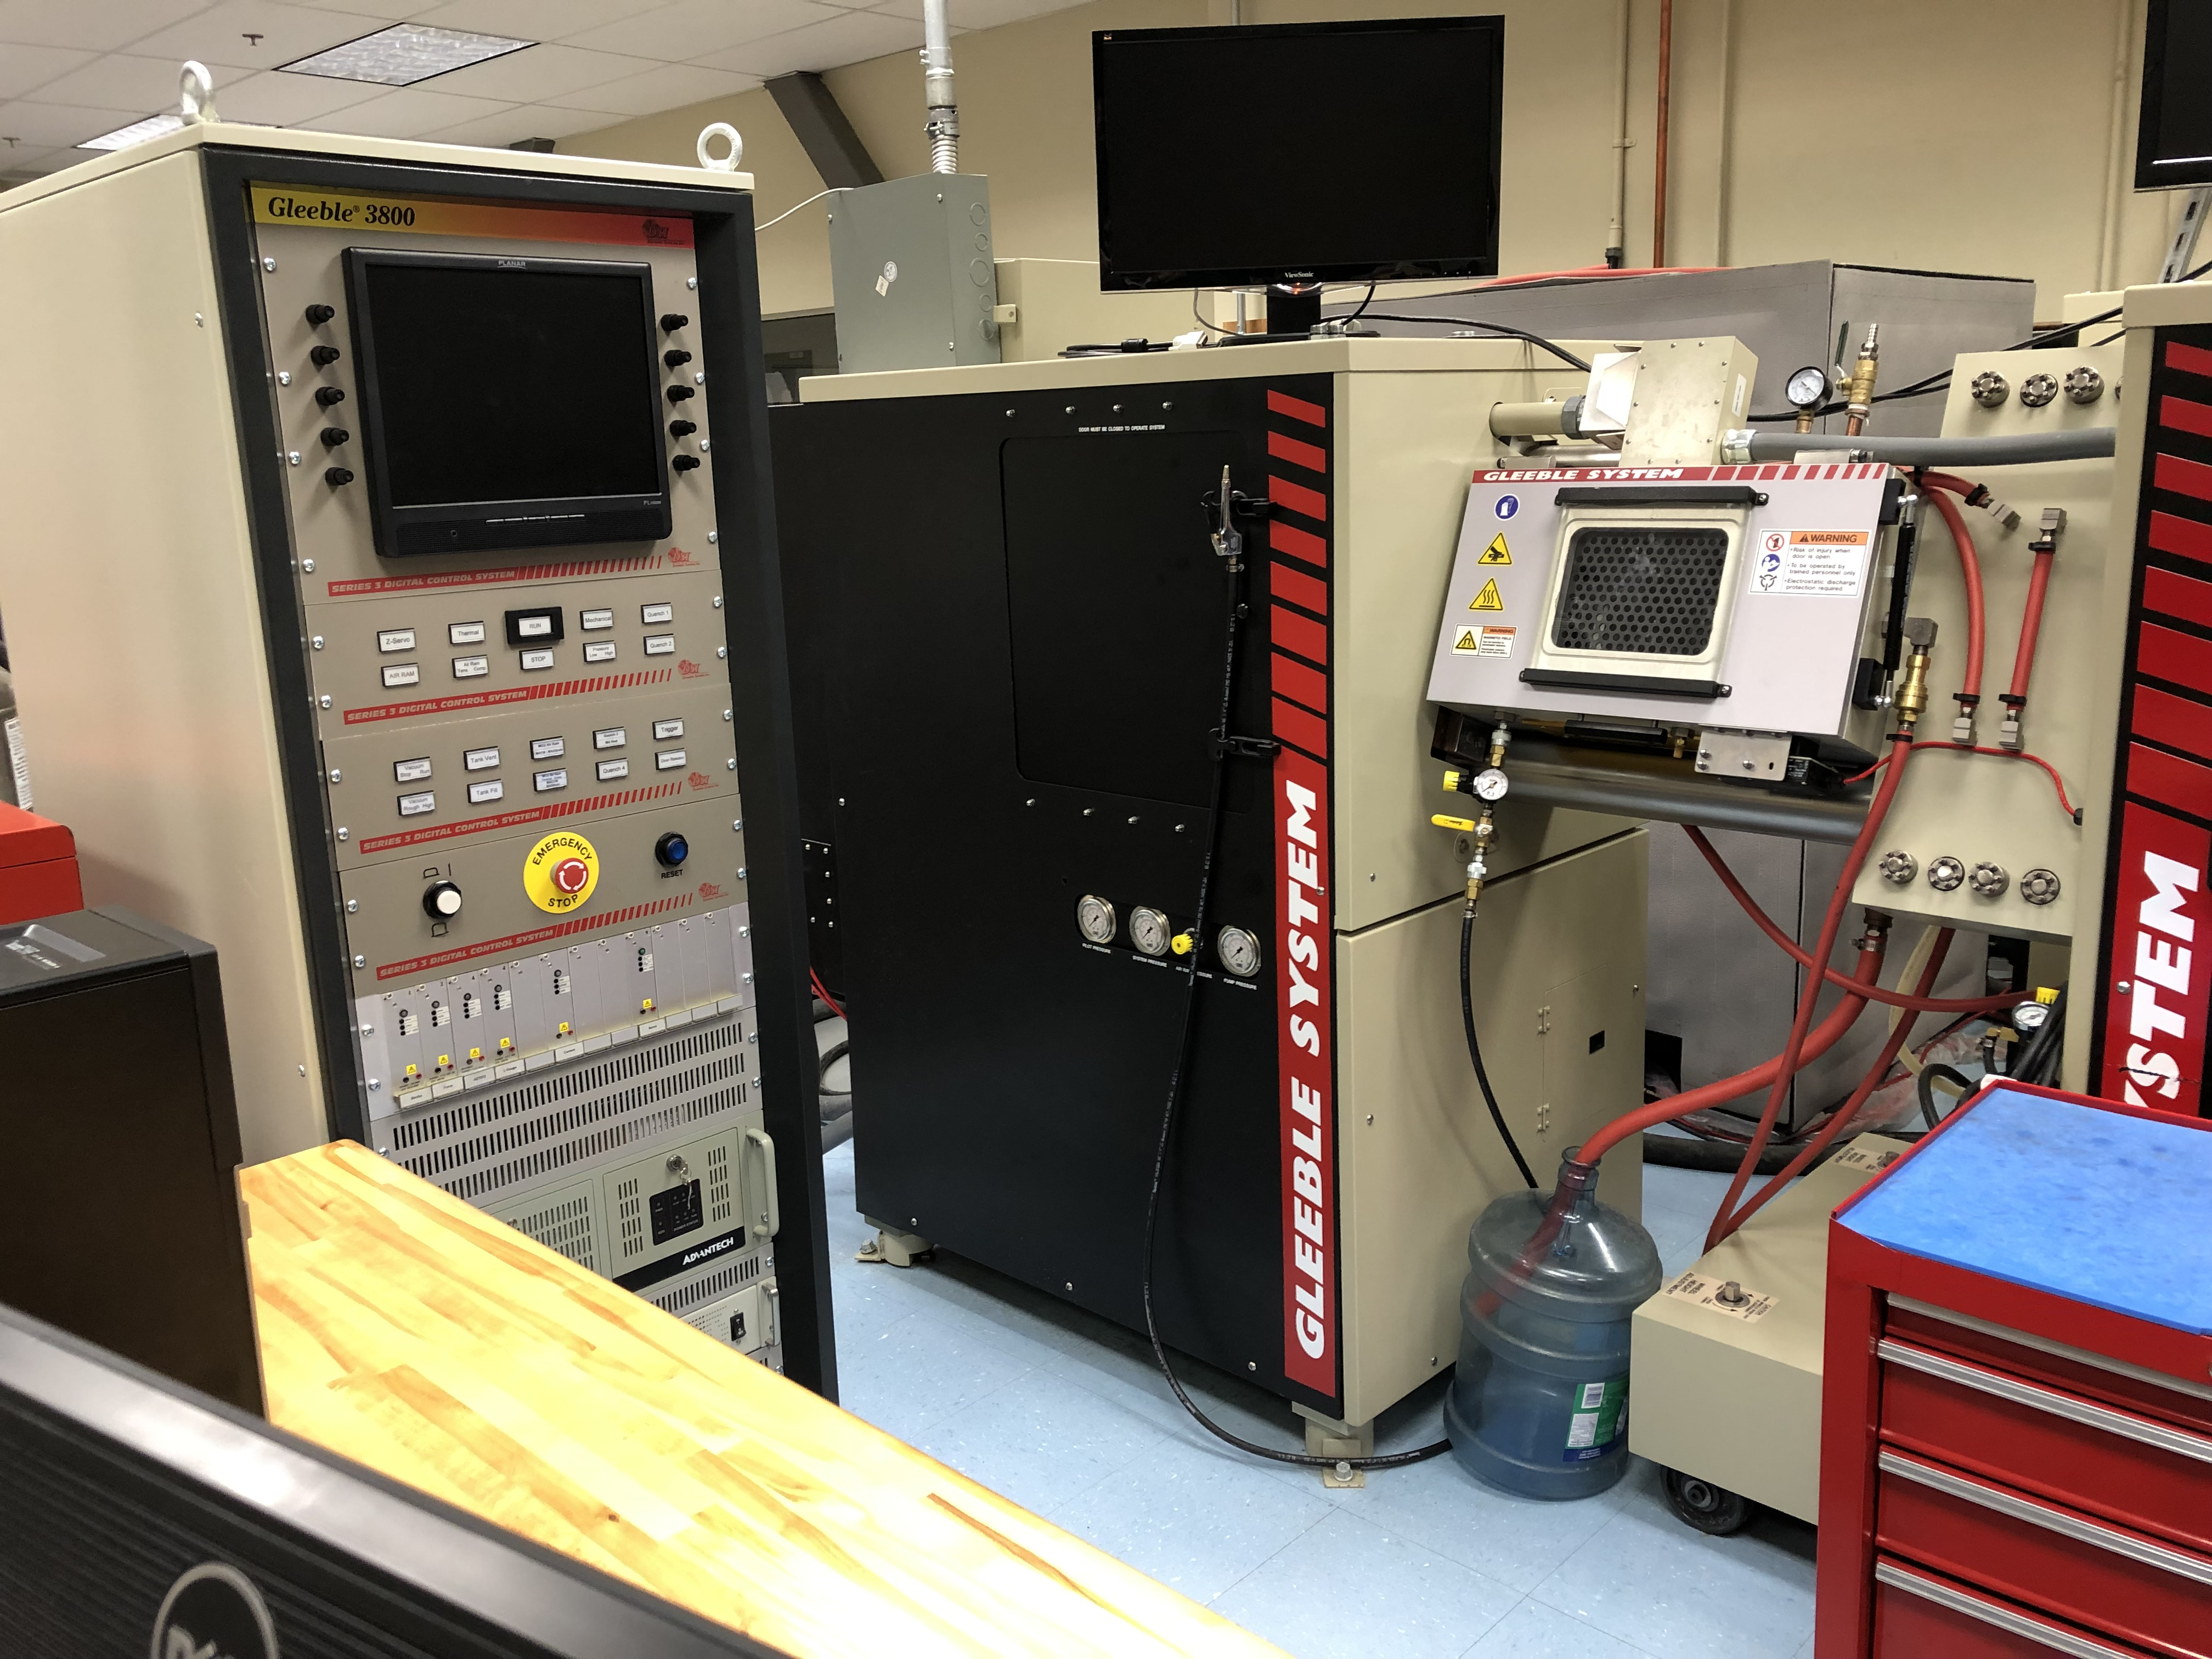
\includegraphics[width=0.7\columnwidth]{Figures/Gleeble-3800}
\caption{The Gleeble-3800 thermomechanical simulator system used for this study}
\label{fig:Gleeble3800}
\end{figure}

Thin tantalum sheets were used as a lubricating material at the contact surface of the anvils and samples to minimize friction during testing.
As shown in Figure \ref{fig:GleebleProcess}, the samples were heated to a temperature of $1260\celsius$ with a heating rate of $2\celsius$/s and held at this temperature for $5$~min to eliminate thermal gradients.
They were then cooled with a rate of $1\celsius$/s to the test temperature and then held at constant temperature for $1$~min before deformation.
During the compression phase, the temperature of the specimen is kept constant by the thermal control system of the machine.
After compression, the specimen is quickly quenched to freeze its microstructure for later analysis.
Figure \ref{fig:GleebleProcess} also shows the aspects of the specimens before and after the compression test: $h_0$ and $R_0$ are the height and radius before compression and $h$, $R_M$ and $R_T$ are the height, large radius and small radius of the specimen after compression, respectively.
\begin{figure}[!ht]
\centering
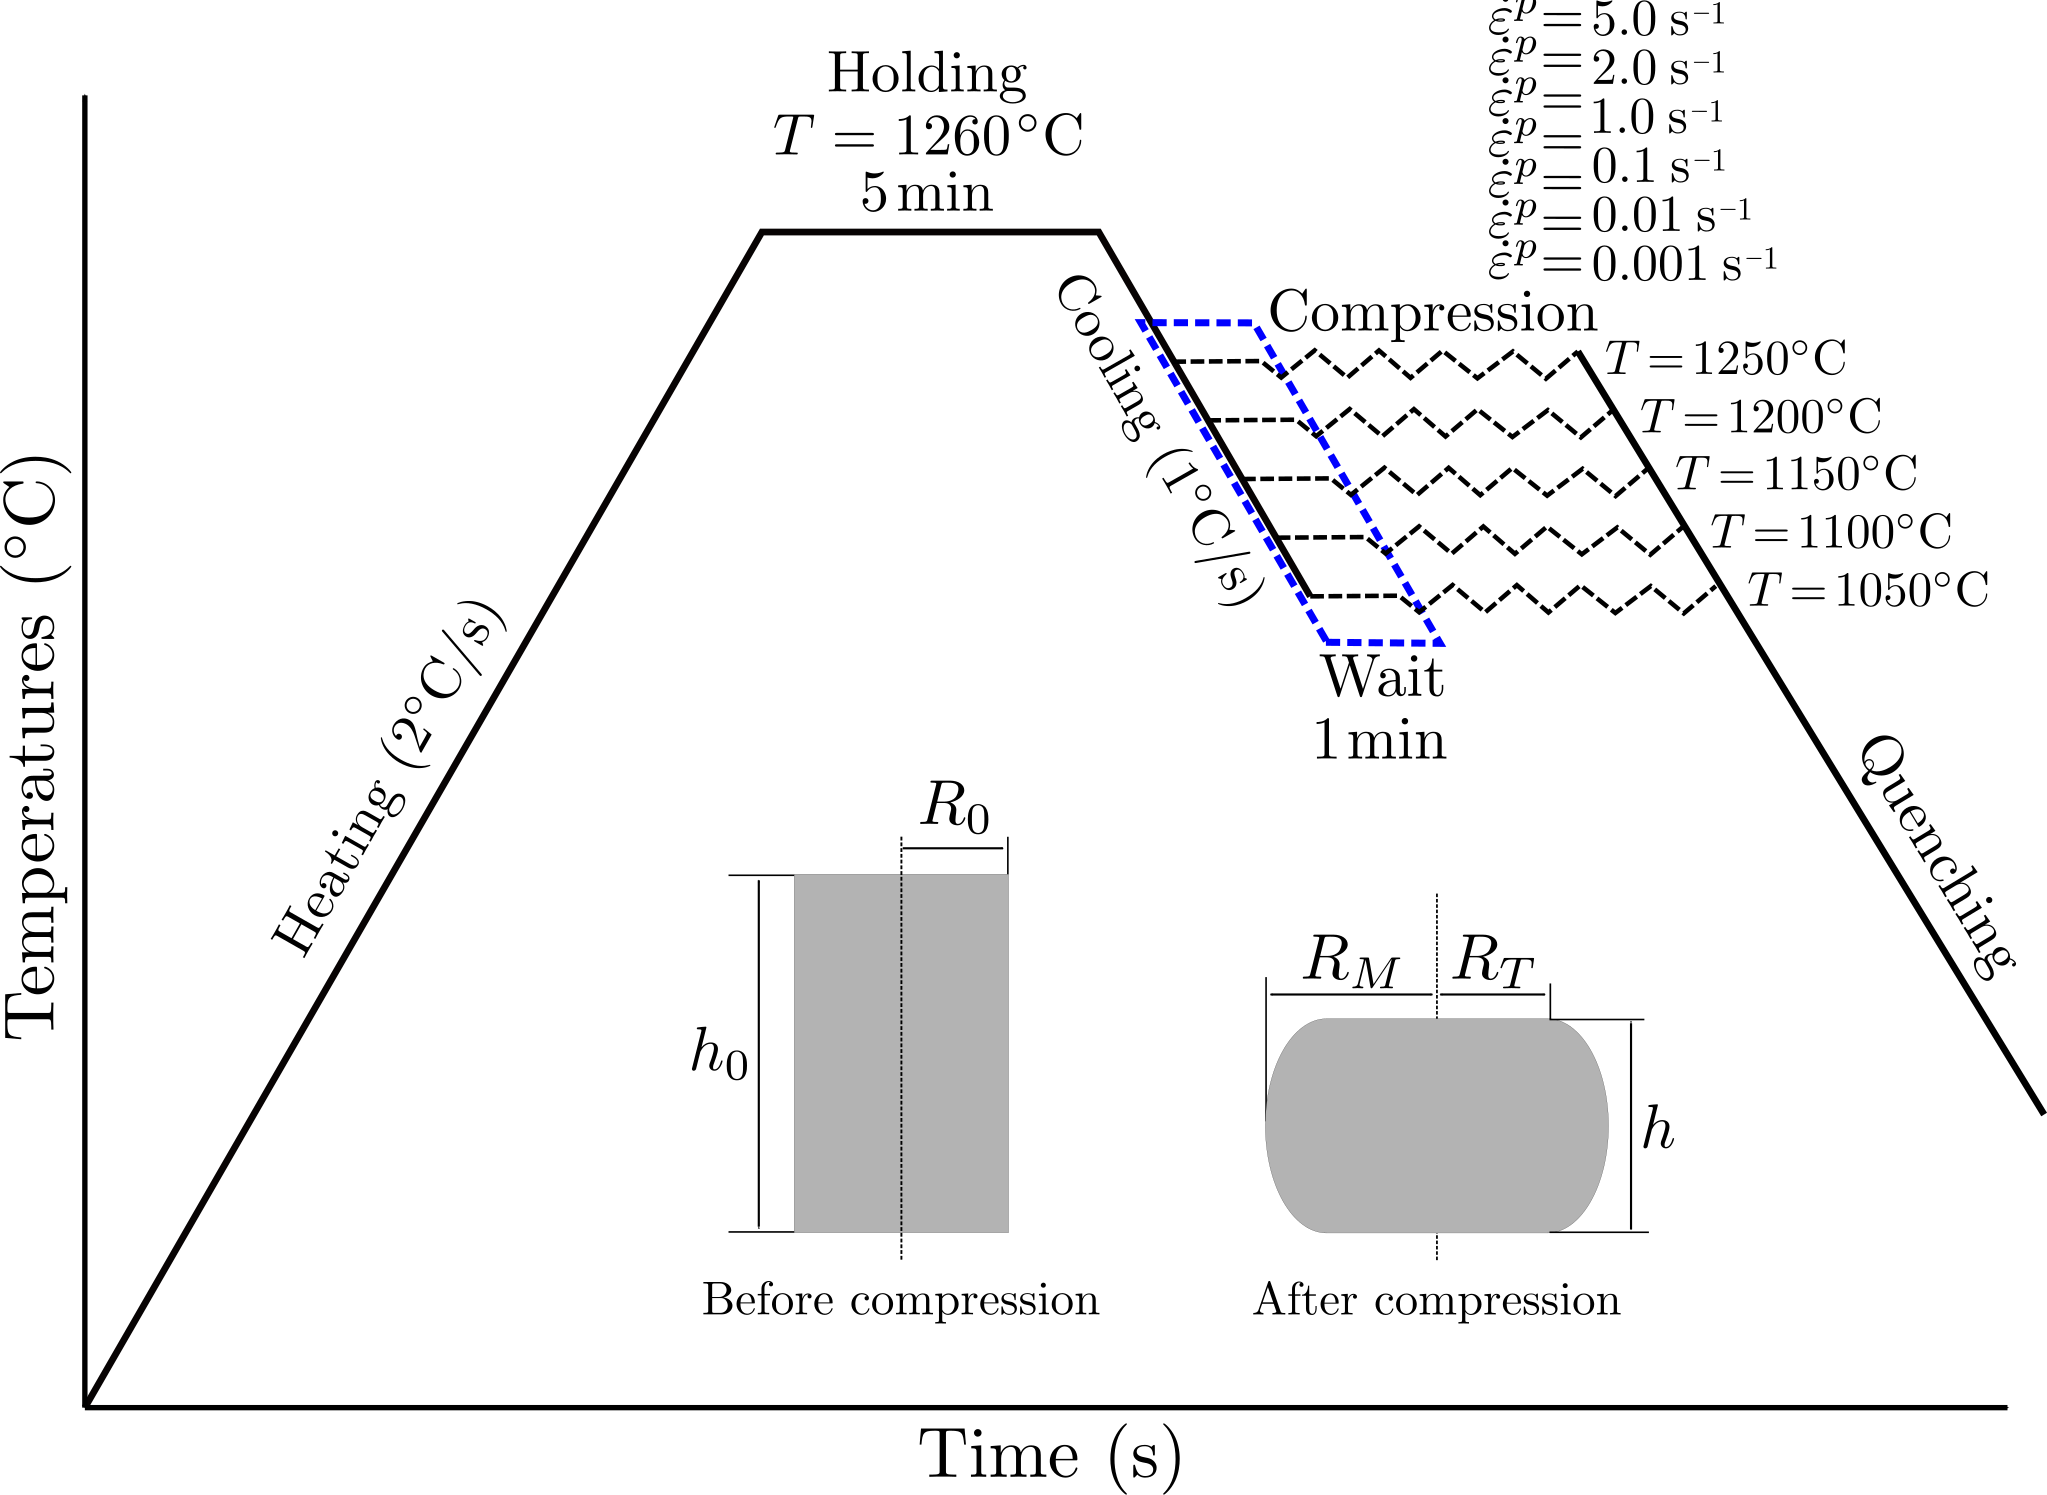
\includegraphics[width=0.8\columnwidth]{Figures/GleebleProcess}
\caption{Schematic diagram of the experimental process.}
\label{fig:GleebleProcess}
\end{figure}

\OP{Here, a part concerning the treatment of the Gleeble data is missing.
You introduce the notions of $h_0$, $R_0$, $h$, $R_M$ and $R_T$ and we have no idea what they are for.
How are the Gleeble data transformed into curves, what is the use of the previous values, what are the corrections to be made to the data,...}\textcolor{red}{The curves are automaticaly gotten from Gleeble system as True-stress and strain according to L-gauge where the formula to get curves are given by $\sigma =F/A\ \text{and}\ \varepsilon = \ln\left(h_0 +\Delta h / h_0\right) $or C-gauge whose formula are $\sigma = 4F/\pi(d+\Delta d)^2$ and $\varepsilon = 2\ln(d/(d+\Delta d))$ with $d = 2R_0$ and $F$ is the force as measured by Gleeble load cell.
As there are noises from raw data, filter method is applied to remove noise and have more smooth data.
For further usage of  data in numerical simulation elastic parts have been removed}.

%------------------------------------------------------------------------
\subsection{Compression tests results\label{sec:ComTestResults}}
%------------------------------------------------------------------------

The set of flow stress $\sigma^y$ versus strain $\varepsilon$ curves obtained from compression tests performed on the Gleeble-3800 simulator for each test condition ($6$ strain rates and $5$ temperatures) is presented in Figure \ref{fig:RawData}.
\OP{It is necessary to give indications concerning the structure of the data: how many points, what amplitude of deformation,...}\textcolor{red}{almost all data are around 21030 or less than and the ammplitude of deformation is between $0.7$ and $0.85$.
We have decided to limit the identification up to $0.7$ because for strain rates $2$ and $5$, stresses are note good}.
The overall behavior of these curves shows that the flow stress $\sigma^y$ increases with increasing strain rate $\mdot\varepsilon$ but decreases with increasing temperature $T$.
It should be noted that the strain also influences the flow stress.
Indeed, for the lowest strain rates $\mdot\varepsilon$, the flow stress $\sigma^y$ increases with the strain $\varepsilon$ until a value of about $\varepsilon=0.2$ to $0.3$, then decreases to maintain a more or less constant value until the end of the test.
For the highest strain rates ($1.0~\ps$, $2.0~\ps$, and $5.0~\ps$), the flow stress increases throughout the test.
One reason for the slight increase in stress at low strain rates when the strain is large is due to friction between the sample and the anvil during the test.
For low strain rates, the effect of lubrication decreases over time and thus friction increases.
This results in a progressive increase of the flow stress.

\begin{figure}[!ht]
\centering
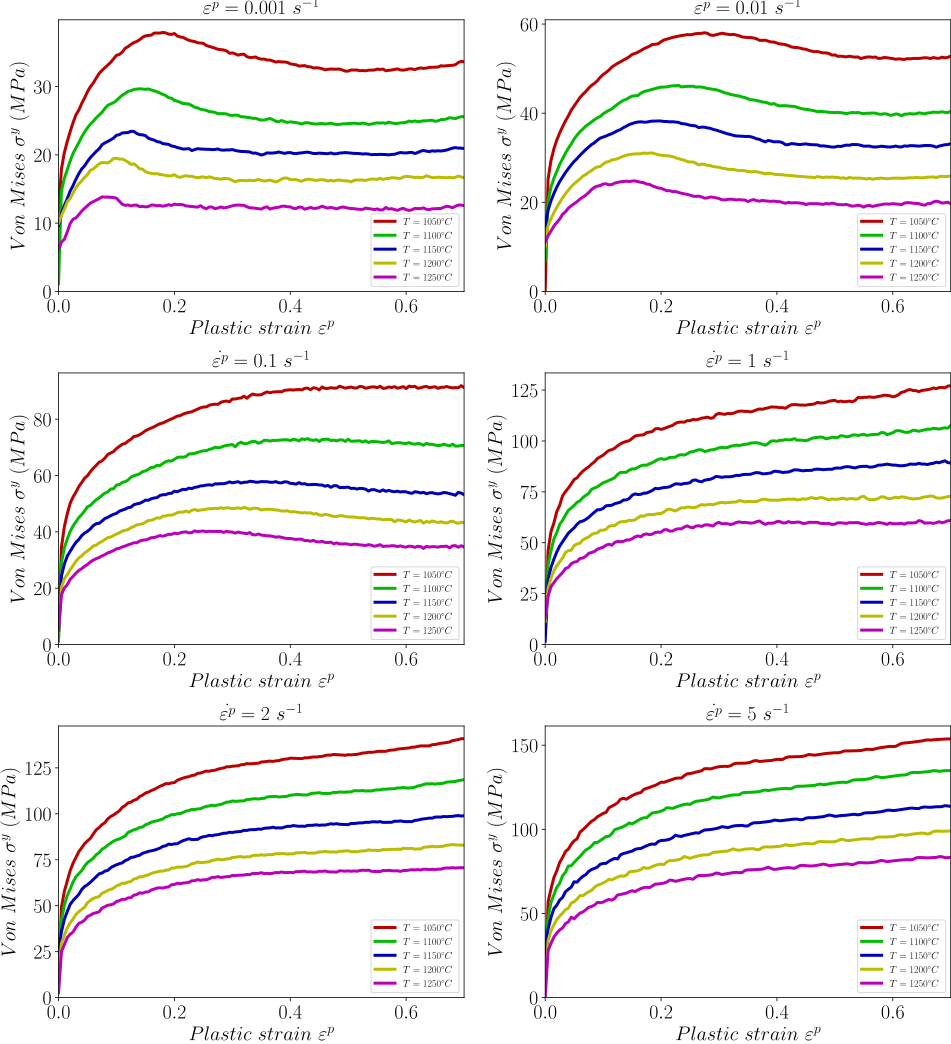
\includegraphics[width=1.02\columnwidth]{Figures/rawData}
\caption{Flow stress-strain curves of AISI P20 alloy at various temperatures and strain rates.}
\label{fig:RawData}
\end{figure}

To explain the overall flow stress behavior observed in this test, we will rely on two fundamental phenomena that can be observed during a compression test: Dynamic Recovery (DRC) and Dynamic Recrystallization (DRX).
At the beginning of the deformation of the sample in compression, the amount of dislocations increases and they begin to move within the material, which leads to a rapid increase in stress (strain hardening phenomenon).
As the strain continues to increase, many dislocations are in motion, leading to a stress relaxation phenomenon, generally known as DRC.
This DRC mechanism contributes to the decrease in the number of dislocations due to their combination with another dislocation or due to their integration into a grain boundary.
Some of these dislocations reorganize and then form sub-grains within the initial grains of the material.
The combination of these dislocations moderates the increase in the number of dislocations related to work hardening and thus controls the amount of strain energy stored in the material, which influences the increase in flow stress.
The dynamic recrystallization concerns the germination of new grains, at the borders or inside the initial grains.
These two phenomena explain the different shapes of the flow stress curves observed for this alloy.
As an example, Figure \ref{fig:Micrography} show the microstructures of AISI P20 held during $5$~min at $1260\celsius$ before and after the compression phase.
As observed on the flow curves, it can be seen by comparing these two micrographs that recrystallization is almost complete for this temperature and strain rate within the sample \textcolor{red}{held for $5$ minutes at $1260^\circ$C and rapidely cooled to get autenized grain in one hand and in other hand held for $1$ minute at $1150^\circ$C before compression with strain rate $0.001\ \text{s}^{-1}$}.
\OP{What are the temperature and strain rate related with this micrography}
From the results reported in Figure \ref{fig:RawData}, the identification of the parameters of the six flow laws proposed in this work will be presented in the next section in order to predict the behavior of the material in any test condition.

\begin{figure}[!ht]
\centering
\begin{subfigure}[b]{0.45\textwidth}
\centering
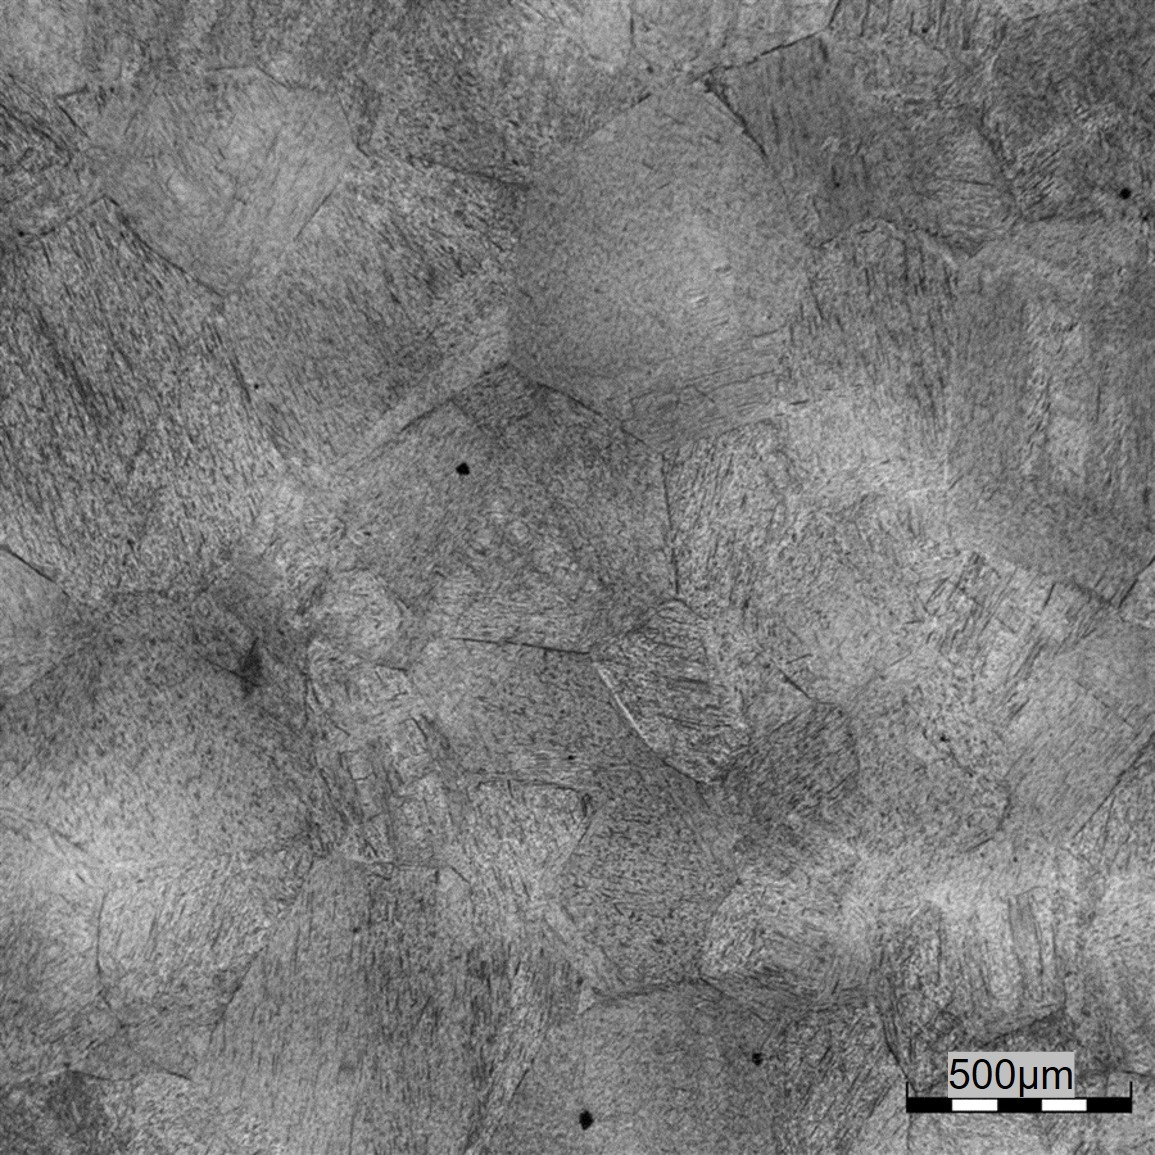
\includegraphics[width=\textwidth]{Figures/BeforeCompM}
\caption{Before hot compression}
\end{subfigure}
\hfill
\begin{subfigure}[b]{0.45\textwidth}
\centering
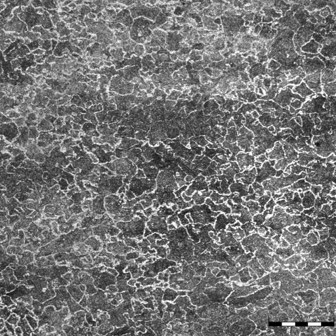
\includegraphics[width=\textwidth]{Figures/AfterCompM}
\caption{After hot compression}
\end{subfigure}
\caption{Optical micrographs of the AISI P20 steel before and after hot compression.}
\label{fig:Micrography}
\end{figure}

%-------------------------------------------------------------------------
\section{Identification of constitutive flow laws parameters\label{sec:ConstLaws}}
%-------------------------------------------------------------------------

The complete characterization of the thermomechanical behavior of a material through the identification of its flow law is very important before its modeling in numerical simulations.
This characterization usually involves experimental tests that serve as a basis for the development of constitutive laws.
As mentioned in the introduction, many constitutive laws exist today, and the selection of one of them on the basis of explicit criteria makes the development of computational models for new materials with new types of behavior challenging.
Since the purpose of this work is to compare the ANN model to analytical models, it is important to justify the choice of analytical models selected for this study among the many that exist in the literature.
Among the analytical models, the Johnson-Cook (JC) model \cite{Johnson-1983} is the most used because of its simplicity of implementation linked to the reduced number of its parameters and the ease to identify them.
It should be noted that it is not the best model but the most integrated in the Finite Elements softwares.
This also explains the existence of several modified forms of this model.
The Zerilli-Armstrong model, and in particular its modified forms (MZA) \cite{NematNasser-2004, Lennon-2004, Muralli-2017, Cheng-2021, Muralli-2021}, is also widely used because it attempts to provide solutions to the shortcomings of the JC model, particularly with regard to the coupling of physical parameters.
It is therefore also part of this study.
The Hansel Spittel (HS) model \cite{Hensel-1978} is also one of the most widely used models in numerical simulation of casting and forging operations because it is natively integrated in the Forge software.
Moreover, the method of identifying its parameters is very simple to perform since it is done in one step.
It also has limitations as we will show in the following sections.
The Arrhenius model was also chosen in this study because it is one of the models that not only provides a good prediction of the flow stress but also takes into account the physical parameter $Q$ (the deformation activation energy coefficient) which is of great importance in the microstructural analyses of materials.
The PTM model \cite{TizeMha-2022} is also used in this study because it is a model whose formulation does not impose a priori a number of parameters and which proved its ability in our previous works.
We selected it to test it on this type of material because it is normally formulated to fit any type of material.

%-------------------------------------------------------------------------
\subsection{Johnson-Cook model\label{sec:JC}}
%-------------------------------------------------------------------------

The JC model, as mentioned above, is one of the most widely used analytical models because it can be applied to many materials under different conditions of strain $\varepsilon$, strain rate $\mdot\varepsilon$, and temperature $T$.
However, the formulation of this model does not take into account the simultaneous effect of strain, strain rate and temperature.
Indeed, it is formulated by describing the effect of each physical parameter ($\varepsilon$, $\mdot\varepsilon$ and $T$) separately as a factor in the mathematical expression of the model.
Hence its inability to describe the phenomenon of softening induced by temperature.
The equation that describes this model is given as follows \cite{Johnson-1983}:

\begin{equation}
\sigma^y=\left(A+B\varepsilon^{p^{n}}\right) \left[1+C\ln\left(\frac{\mdot\varepsilon}{\mdot\varepsilon_0}\right)\right] \left[1-\left(\frac{T-T_0}{T_m-T_0}\right)^{m}\right],\label{eq:Johnson-Cook}
\end{equation}
where $\sigma^y$ is the flow stress, $\varepsilon^p$ is the plastic strain, $A$ is the initial elastic limit of the material, $B$ is the strain hardening coefficient, $n$ is the strain hardening exponent, $C$ and $m$ are the material constants that describe the strain rate hardening coefficient and the thermal softening coefficient, respectively.
The other values are reference ones, so that $\mdot\varepsilon_0$ is the reference strain rate, $T_m$ and $T_0$ are the melting temperature ($1460\celsius$ in our case) and the reference temperature, respectively.

For the determination of the parameters of the analytical models, the reference values for strain rate and temperature are $\mdot\varepsilon_0=0.001~\ps$ and $T_0=1050\celsius$ respectively.

The procedure used for the determination of the parameters of the Johnson-Cook law is in accordance with the one proposed by He \eal \cite{He-2013}.
This method allows obtaining one after the other the $5$ parameters in the order $A$, $B$, $n$, $C$ and $m$.
Thus, according to the experimental data, the initial elastic limit of the material at the reference strain rate and reference temperature is $A=13.5143$~MPa.
For the determination of the constants $B$ and $n$, from the results of the compression test at $T_0$ and $\mdot\varepsilon_0$, it is then possible to determine these two constants by considering only the first term $\left(A+B\varepsilon^{p^{n}}\right)$ in Equation (\ref{eq:Johnson-Cook}).
Thus, here, $B=21.816$~MPa and $n=0.0746$.
Once the parameters $A$, $B$ and $n$ are known, the determination of $C$, considering all the curves at $T=T_0$ then gives $C=0.3404$.
Finally, the last parameter $m$ is identified from the curves at $\mdot\varepsilon=\mdot\varepsilon_0$ and from the knowledge of the previous and gives $m=0.7057$.
All parameters of the Johnson-Cook model are reported in Table \ref{tab:JC}.

\begin{table}[h!]
\centering
\caption{Parameters' values of the Johnson-Cook flow law for the P20 steel.}
\begin{tabular}{ccccc}
\hline
$A~(\text{MPa})$ & $B~(\text{MPa})$ & $n$ & $C$ & $m$\\
$13.5143$&$21.816$&$0.0746$&$0.3404$&$0.7057$\\ \hline
\label{tab:JC}
\end{tabular}
\end{table}

The values predicted by the Johnson-Cook flow law (solid line) and the experimental values (dots) are compared in Figure \ref{fig:CompExp-JC-6}.
The JC model is not able to describe the evolution of the flow stress of AISI P20 for all strain values, and the predicted stresses $\sigma^y$ show a monotonically decreasing trend for several values of the strain rates.
The discrepancy between the predicted and experimental values is large for low strains and sometimes acceptable for high strains.
As expected, the mathematical formulation of the Johnson-Cook flow law is unable to represent the stress drop at low strain rates, the JC model being only monotonically increasing with strain.
Since most of the parameters are identified at low strain rates ($A$, $B$ and $n$), this results in a very poor fit of the model to the experimental data.

\begin{figure}[!ht]
\centering
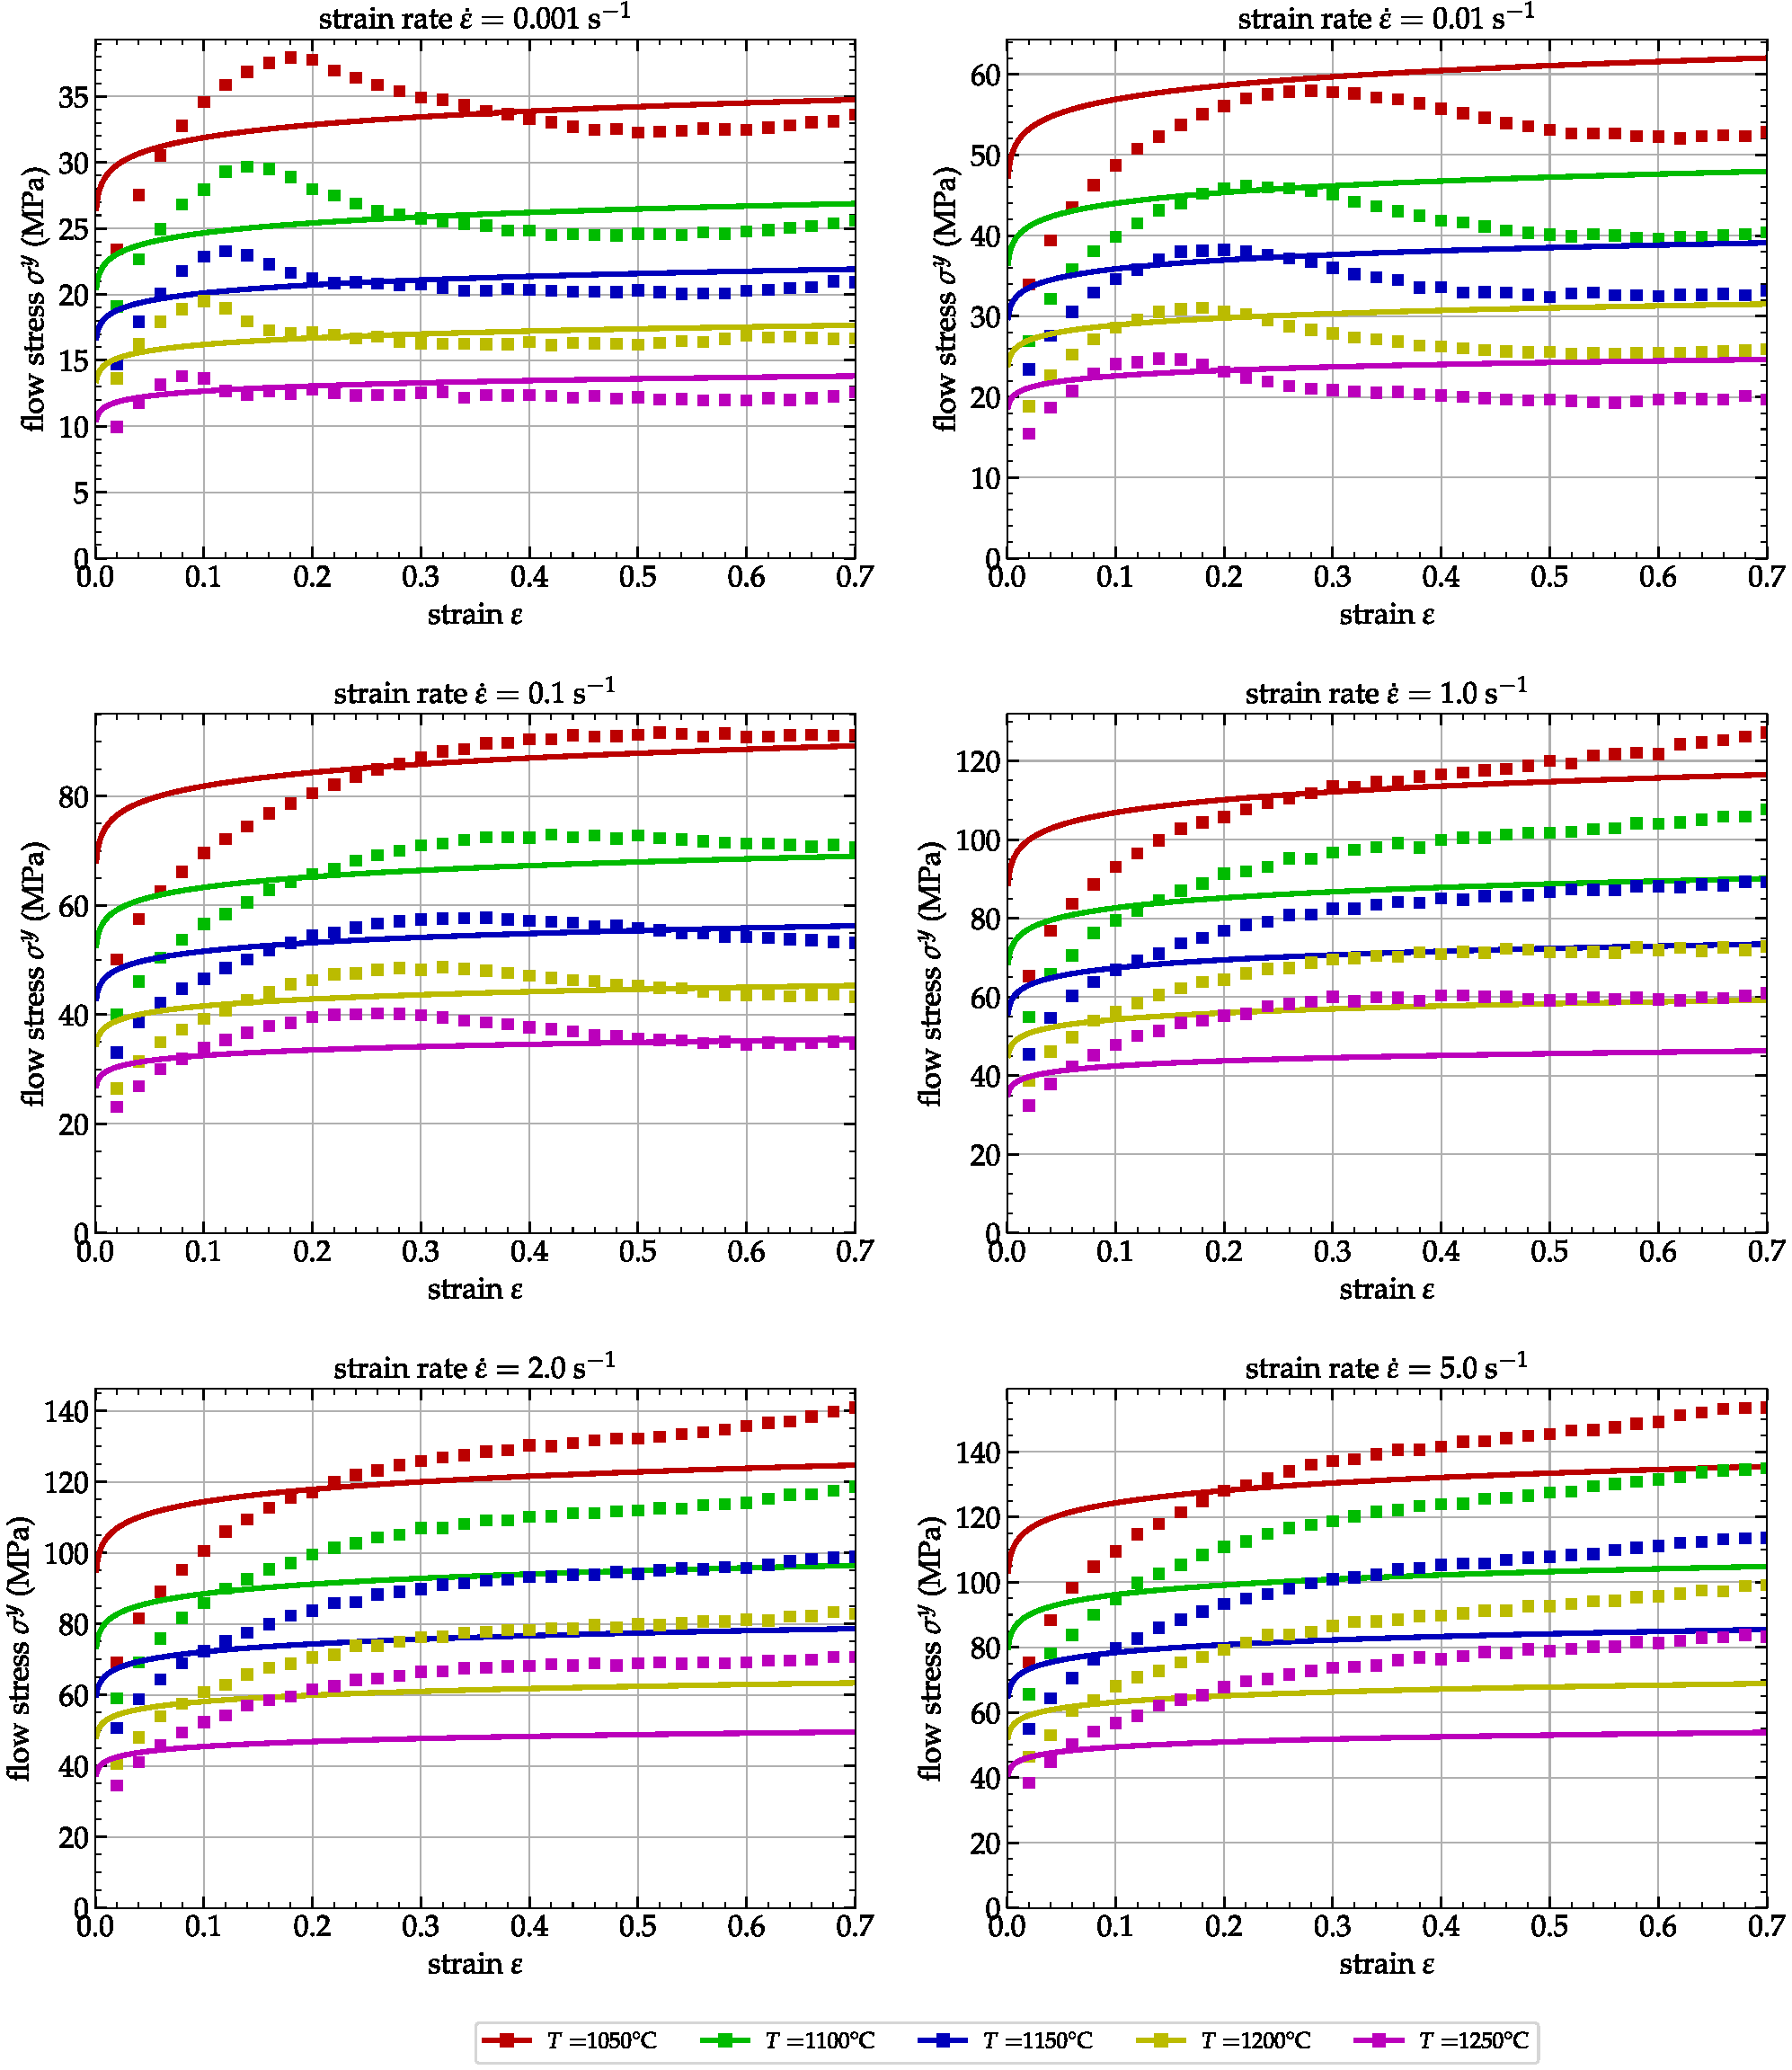
\includegraphics[width=1.02\columnwidth]{Figures/CompExp-JC-6}
\caption{Comparison between the experimental and predicted flow stresses by JC model.}
\label{fig:CompExp-JC-6}
\end{figure}

The accuracy and predictive ability of the models are usually assessed by certain coefficients such as the Mean Absolute Relative Error ($\AARE$) defined by Equation (\ref{eq:AARE}) and the Root Mean Square Error ($\RMSE$) defined by Equation (\ref{eq:RMSE}).
\begin{equation}
\AARE(\%) = \frac{1}{N} \sum_{i=1}^{N}{\left|\frac{\sigma_i^p -\sigma_i^e}{\sigma_i^e}\right|} \times 100 \label{eq:AARE}
\end{equation}
\begin{equation}
\RMSE (\text{MPa}) = \sqrt{\frac{1}{N} \sum_{i=1}^{N} \left(\sigma_i^p - \sigma_i^e\right)^2} \label{eq:RMSE}
\end{equation}
where $\sigma_i^e$ is the experimental value and $\sigma_i^p$ is the predicted value using the given model of the flow stress $\sigma^y$ and $N$ is the total number of data points used to compute those coefficients (in our case $N=21000$).
For the JC model, $\AARE=14.05~\%$ and $\RMSE=12.00~\text{MPa}$.
The correlation coefficient ($R$) is generally not a good measure in our case of study because it only shows the correlation of the model with respect to the data and not its accuracy, which is a determining factor in the qualification of a model.
Therefore, a good (high) value of $R$ (close to $1$) does not necessarily mean a good prediction of the model but simply establishes a good linearity correlation between the experiment and the prediction \cite{Phaniraj-2003}.

%-------------------------------------------------------------------------
\subsection{Modified Zerilli-Armstrong model\label{sec:MZA}}
%-------------------------------------------------------------------------
\OP{This introduction paragraph is entirely copied from the WJET publication, P.T.M.
must rewrite this part of the text !}
\textcolor{red}{The MZA which is the modified form of ZA model, as the JC model is one of widely used models and implemented in many sofwares like Abaqus.
The difference between the MZA model and JC model is related to the consideration of the three physical parameters to describe the reality observed from experimental.
Indeed, in the JC model, those parameters are considered separately where they are simultaneaously considered in MZA and for that formulation MZA is prefered to JC model} \cite{Hull-2011}.
But the original form of ZA model has some limitations due to the fact that it is considered as two terms and to ameliorate that formulation Samantaray \eal \cite{Samantaray-2009} proposed a modified form given by the following equation:
\begin{equation}
\label{eq:MZA-model}
\sigma^y = \left(C_{1}+C_{2}\varepsilon^{p^n}\right) \exp\left[-\left(C_{3}+C_{4}\varepsilon^p\right)\left(T-T_0\right) + \left(C_{5}+C_{6}\left(T-T_0\right)\right)\ln\left( \frac{\mdot\varepsilon}{\mdot{\varepsilon}_0}\right)\right]
\end{equation}
where the $7$ coefficients $C_i$ and $n$ are the parameters of the model to be identified for a given material.
The formulation of the model can be found in \cite{Samantaray-2009} and determination of its parameters is sumarized as following.

Considering the expression of the model given by Equation (\ref{eq:MZA-model}), parameter $C_1$ is deduced direcly from $\sigma^y(\varepsilon^p=0,T=T_0,\mdot\varepsilon=\mdot{\varepsilon}_0)$.
When the current strain rate $\mdot\varepsilon$ is identical to the reference strain rate $\mdot{\varepsilon}_0$, the Equation (\ref{eq:MZA-model}) becomes :
\begin{equation}
\sigma^y = \left(C_{1}+C_{2}\varepsilon^{p^n}\right) \exp\left[-\left(C_{3}+C_{4}\varepsilon^p\right)\left(T-T_0\right)\right]
\end{equation}
Taking the logarithm of the previous relationship we have :
\begin{equation}
\ln\sigma^y = \ln\left(C_{1}+C_{2}\varepsilon^{p^n}\right)-\left(C_{3}+C_{4}\varepsilon^p\right)\left(T-T_0\right)
\end{equation}
By plotting the function $\ln\sigma^y\left(T-T_0\right)$ the y-intercept and the slope of this line can be deduced as $I_1=\ln\left(C_1+C_2\varepsilon^{p^n}\right)$ and $S_1=-\left(C_3+C_4\varepsilon^p\right)$.
From the expression of $I_1$ we can write:
\begin{equation}
\ln\left(\exp(I_1)-C_1\right) = \ln C_2+n\ln\varepsilon^p
\end{equation}
By plotting the function $\ln\left(\exp(I_1)-C_1\right)$ versus $\ln\varepsilon^p$ we can deduce $n$ and $C_2$.
The plot of $S_1$ versus $\varepsilon^p$ allows deducing $C_3$ and $C_4$ from the y-intercept and the slope, respectively.
Once the first four terms of the model are calculated, we can now take the logarithm of the entire MZA model given by Equation (\ref{eq:MZA-model}).
\begin{equation}
\ln\sigma^y = \ln\left(C_{1}+C_{2}\varepsilon^{p^n}\right) - \left(C_{3}+C_{4}\varepsilon^p\right)\left(T-T_0\right) + S_2\ln\left( \frac{\mdot\varepsilon}{\mdot{\varepsilon}_0}\right)
\end{equation}
with $S_2=C_5+C_6\left(T-T_0\right)$.
Finally, the graph $\ln\sigma^y$ versus $ \ln(\mdot\varepsilon/\mdot{\varepsilon}_0)$ allows deducing $C_5$ and $C_6$ from the slope $S_2$.
The parameters of MZA model are given in the Table \ref{tab:MZA} while its prediction are shown in Figure \ref{fig:CompExp-MZA-6}.
It can be seen from those figures that the MZA model as JC model is not suitable to describe experimental at low strain rates but much better for high strain rates.
The deviation between the predicted values and the experimental values is large because this model has problem to correctly describe the softening in its formulation.
For the MZA model, $\AARE=21.20~\%$ and $\RMSE=19.57~\text{MPa}$, this shows an overall worse performance than the JC model.
That is aspect of the limitations of that model as presented in \cite{TizeMha-2022}.
\begin{table}[h!]
\centering{}
\caption{Parameters' constants of Modified-Zerilli-Armstrong Model}
\begin{tabular}{ccccccc}
\hline
$C_1$ & $C_2$ & $C_3$ & $C_4$ & $C_5$ & $C_6$ & $n$\\
$13.5143$ & $21.2591$ & $4.7902\times 10^{-3}$ & $1.4895\times 10^{-4}$ & $0.1389$ & $1.495\times 10^{-4}$ & $0.0621$\\
\hline
\label{tab:MZA}
\end{tabular}
\end{table}
\begin{figure}[!ht]
\centering
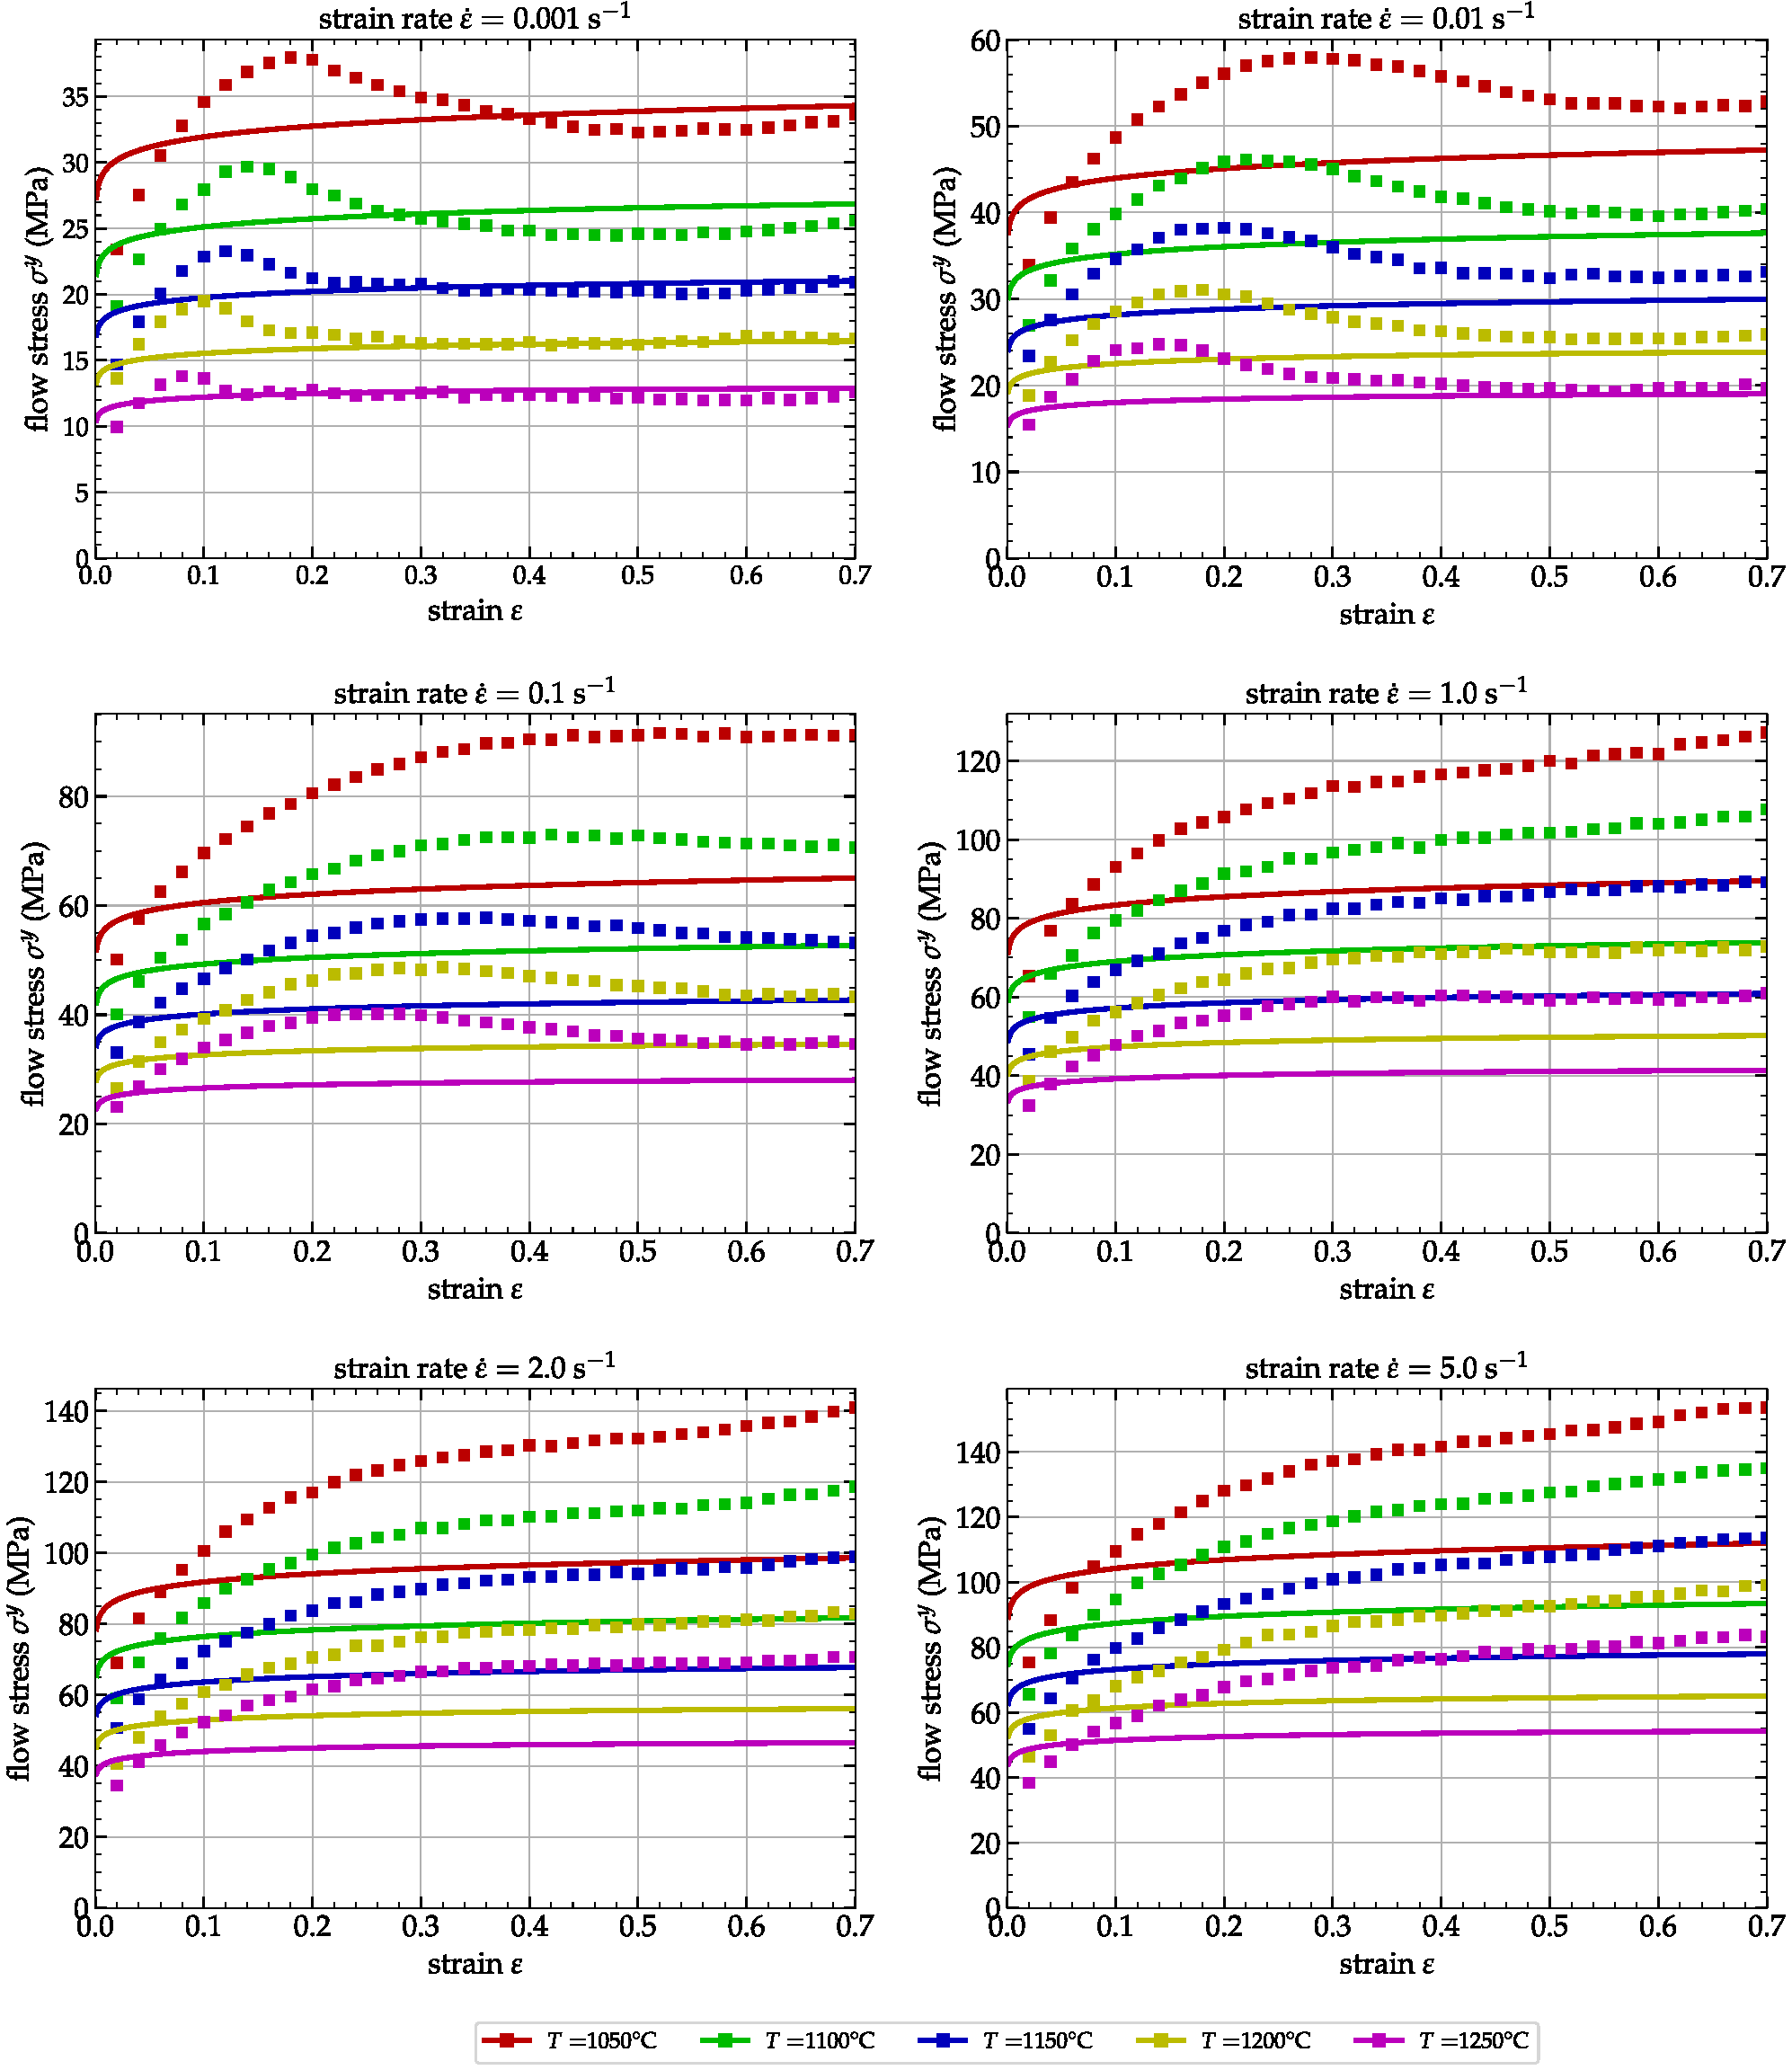
\includegraphics[width=1.02\columnwidth]
{Figures/CompExp-MZA-6}
\caption{Comparison between the experimental and predicted flow stresses by MZA model}
\label{fig:CompExp-MZA-6}
\end{figure}

%-------------------------------------------------------------------------
\subsection{Hansel and Spittel model\label{sec:HSmodel}}
%-------------------------------------------------------------------------

The Hansel-Spittel model \cite{Hensel-1978} is one of the least known models in terms of integration in finite element simulation software, although the determination of its parameters is easier than that of the JC or MZA model.
The programming of a simple identification script is sufficient to identify its parameters for a given material.
The equation of the HS model is given by the following relation:
\begin{equation}
\sigma^y = A~\e{m_1T}~\varepsilon^{m_2}~\mdot\varepsilon^{m_3}~\e{({m_4}/{\varepsilon})}~(1+\varepsilon)^{m_5T}~\e{m_6\varepsilon}~\mdot\varepsilon^{m_7T}~T^{m_8} \label{eq:HS}
\end{equation}
where $\sigma^y$ is the flow stress, $\varepsilon$ is the strain, $\mdot\varepsilon$ is the strain rate and $T$ is the temperature as proposed earlier.
The coefficients $A$ and $m_i$ are the parameters of the model to be identified.
However, this model has some shortcomings, notably related to the fact that its accuracy varies according to the number of parameters taken into account during the identification.
For its identification, several authors restrict its expression to a reduced number of $5$ or $6$ $m_i$ parameters only, by forcing a zero value for the other parameters \cite{Chadha-2018, Rudnytskyj-2020, Mehtedi-2015}.

In the present study, the best results were obtained by taking the model defined by only the first $7$ $m_i$ terms of the equation (\ref{eq:HS}), so that $m_8=0$.\OP{See identification script for changes}
From the experimental data obtained during the compression tests, an identification procedure based on the use of the LMFIT optimizer \cite{Newville-2016} has allowed to compute the parameters reported in Table \ref{tab:HS}.

\begin{table}[h!]
\centering
\caption{Parameters' values of the Hansel-Spittel flow law for the P20 steel.}
\begin{tabular}{ccccc}
\hline
$A$ & $m_1$ & $m_2$ & $m_3$ & $m_4$\\
$5.954\times 10^{3}$ & $-3.3576\times10^{-3}$ & $0.2641$ & $-0.0868$ & $2.2688\times10^{-4}$\\\hline
& $m_5$ & $m_6$ & $m_7$ & $m_8$\\
& $-4.2163\times10^{-4}$ & $-0.0561$ & $2.264\times10^{-4}$ & $0$\\\hline
\label{tab:HS}
\end{tabular}
\end{table}

The comparison of the values predicted by the HS model and the experimental values is presented in Figure \ref{fig:CompExp-HS-6} where the dots represent the experimental values and the solid lines are the values predicted by the Hansel-Spittel flow law.
For the HS model, $\AARE=7.75~\%$ and $\RMSE=3.80~\text{MPa}$.
It appears that this model as well as the previous ones do not predict well the experimental one and the difference is relatively important for all strain rates below $1.0~\ps$.
This shows that this model is not appropriate for the characterization of this alloy, in particular because of the strong non-linearity of the behavior for low values of the strain rate.
The DRX phenomena cannot be reproduced by this type of model.

\begin{figure}[!ht]
\centering
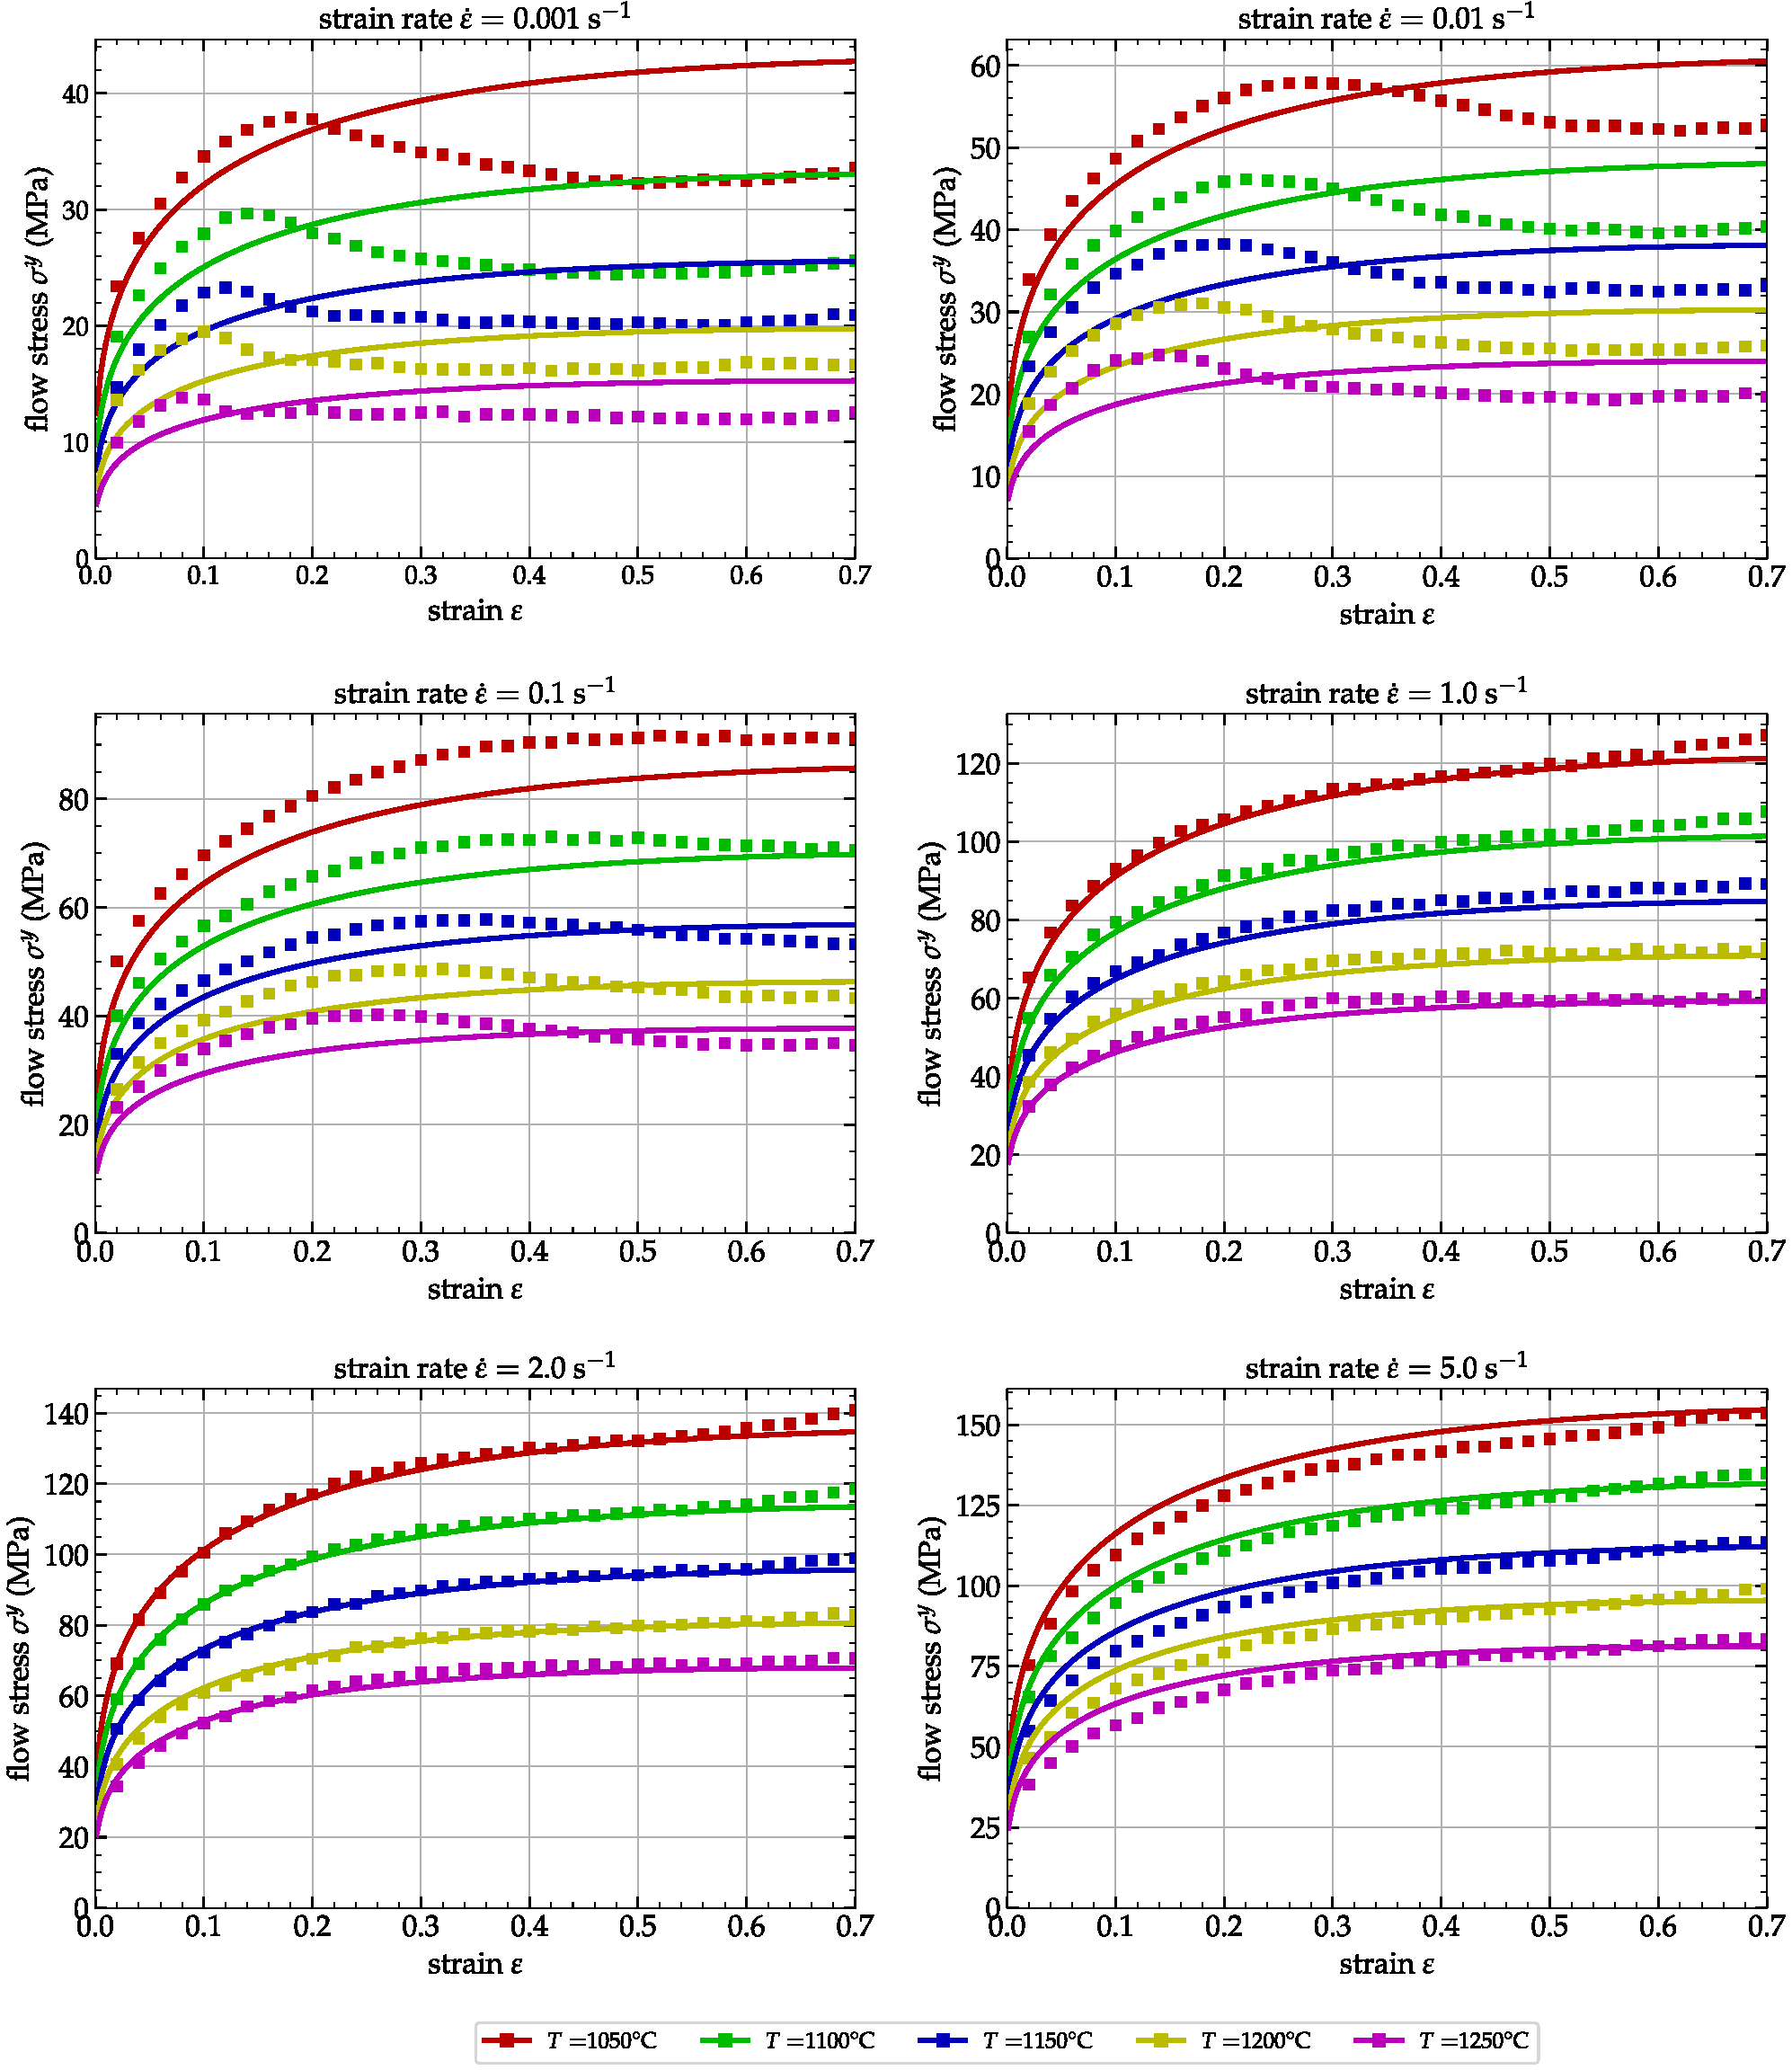
\includegraphics[width=1.02\columnwidth]
{Figures/CompExp-HS-6}
\caption{Comparison between the experimental and predicted flow stresses by HS model}
\label{fig:CompExp-HS-6}
\end{figure}

%----------------------------------------------------------------------------------
\subsection{Arrhenius model\label{sec:ARmodel}}
%----------------------------------------------------------------------------------

The Arrhenius type model \cite{Sellars-1966} is one of the most used models in the framework of material forming, especially when it comes to studying the microstructure of the material.
Indeed, this model takes into account the physical phenomena that describe the behavior of the material in the formulation of the relationships between the stress $\sigma^y$, the strain $\varepsilon$, the strain rate $\mdot\varepsilon$ and the temperature $T$ expressed as power law, exponential law and hyperbolic sine.
This makes it easier to describe the softening phenomenon observed in the material due to increasing temperature.
The following equations describe the Arrhenius model:
\begin{equation}
\mdot\varepsilon =
\begin{cases}
A_1 \sigma^{y^{n_1}} \exp{\left(-\frac{Q}{RT}\right)} & \alpha\sigma^y < 0.8\\
A_2 \exp(\beta\sigma^y) \exp{\left(-\frac{Q}{RT}\right)} & \alpha\sigma^y > 1.2\\
A_3 \left[\sinh{\left(\alpha\sigma^y\right)}\right]^{n_2} \exp{\left(-\frac{Q}{RT}\right)} & \text{for all }\sigma^y
\end{cases}
\label{eq:ArDef}
\end{equation}
with:
\begin{equation}
Z = \mdot\varepsilon \exp{\left(\frac{Q}{RT}\right)} \label{eq:ArZ}
\end{equation}
where $Z$ is the Zenner-Hollomon parameter \cite{Zener-1944}, $\mdot\varepsilon$ is the strain rate ($\ps$), $Q$ is the apparent activation energy ($\text{J~mol}^{-1}$), $R$ is the universal gas constant ($8.314~\text{J~mol}^{-1} \text{K}^{-1}$), $T$ is the absolute temperature (K), $\sigma^y$ is the flow stress (MPa) for a given strain, strain rate and temperature and $A_1$, $A_2$, $A_3$, $n_1$, $n_2$, $\alpha$ and $\beta=\alpha n_1$ are dependent of the material.
The corresponding values are independent of the temperature and are obtained from the stress-strain curves at different strain rates and temperature by regression method.
Combination of Equations (\ref{eq:ArDef}) and (\ref{eq:ArZ}) allow expressing the flow stress $\sigma^y$ as a function of the $Z$ parameter:
\begin{equation}
\sigma^y = \frac{1}{\alpha} \ln\left\{\left(\frac{Z}{A}\right)^{1/n} + \left[1 + \left(\frac{Z}{A}\right)^{2/n}\right]^{1/2}\right\}
\end{equation}

To obtain the constitutive equation, it is necessary to determine all the parameters $A$, $Q$ $\alpha$ and $n$ for a given material.
The strain has a significant non-linear influence on the behavior of the material by the mechanism of strain hardening and softening at high values of deformation.
A compensation in strain must therefore be taken into account in the Arrhenius model, which leads to the definition of the modified Arrhenius model for which the $A$, $Q$ $\alpha$ and $n$ parameters are expressed as a function of the strain $\varepsilon$ by means of polynomial functions of degree $m$ (varying from $1$ to $9$) of the form:
\begin{equation}
A(\varepsilon) = \exp{\left[\ln\!A_0 + \ln\!A_1\varepsilon + \ln\!A_2\varepsilon^2 + \ln\!A_3\varepsilon^3 + \cdots + \ln\!A_m\varepsilon^m\right]}
\label{eq:ArA}
\end{equation}
\begin{equation}
Q(\varepsilon) = Q_0 + Q_1\varepsilon + Q_2\varepsilon^2 + Q_3\varepsilon^3 + \cdots + Q_m\varepsilon^m
\label{eq:ArQ}
\end{equation}
\begin{equation}
\alpha(\varepsilon) = \alpha_0 + \alpha_1\varepsilon + \alpha_2\varepsilon^2 + \alpha_3\varepsilon^3 + \cdots + \alpha_m\varepsilon^m
\label{eq:Aralpha}
\end{equation}
\begin{equation}
n(\varepsilon) = n_0 + n_1\varepsilon + n_2\varepsilon^2 + n_3\varepsilon^3 + \cdots + n_m\varepsilon^m
\label{eq:Arn}
\end{equation}

The determination of the order $m$ of the polynomials defined by Equations (\ref{eq:ArA}-\ref{eq:Arn}) is defined according to the ability of the model to represent the non-linear dependence of the stress versus the strain and its generalization.
The values $\ln\!A_i$, $\alpha_i$, $n_i$, and $Q_i$ ($i=1,2,3,\cdots,m$) are the coefficients of the polynomials to determine using a regression method.
Setting $m=9$ gives the best results and the corresponding parameters are reported in Table \ref{tab:AR}.
\begin{table}[h!]
\centering
\caption{Parameters' values of the Arrhenius flow law for the P20 steel}
\begin{tabular}{llll}
\hline
\multicolumn{1}{c}{$\alpha_i$} & \multicolumn{1}{c}{$Q_i~(\times 10^{-6})$} & \multicolumn{1}{c}{$\ln\!A_i$} & \multicolumn{1}{c}{$n_i$}\\
\hline
$\alpha_0=0.0407$ & $Q_0=0.467$ & $A_0=35.8092$ & $n_0=4.8217$\\
$\alpha_1=-0.5167$ & $Q_1=-0.6517$ & $A_1=-58.822$ & $n_1=3.2814$\\
$\alpha_2=6.3912$ & $Q_2=7.6084$ & $A_2=740.3303$ & $n_2=71.5963$\\
$\alpha_3=-47.3364$ & $Q_3=-48.016$ & $A_3=-5.0493\times 10^{3}$ & $n_3=-1.9562\times 10^{3}$\\
$\alpha_4=220.0014$ & $Q_4=66.795$ & $A_4=1.1305\times 10^{4}$ & $n_4=1.4461\times 10^{4}$\\
$\alpha_5=-654.4553$ & $Q_5=468.8898$ & $A_5=2.022\times 10^{4}$ & $n_5=-5.431\times 10^{4}$\\
$\alpha_6=1.2421\times 10^{3}$ & $Q_6=-2.3032\times 10^{3}$ & $A_6=-1.5387\times 10^{5}$ & $n_6=1.1761\times 10^{5}$\\
$\alpha_7=-1.4523\times 10^{3}$ & $Q_7=4.3707\times 10^{3}$ & $A_7=3.1798\times 10^{5}$ & $n_7=-1.4882\times 10^{5}$\\
$\alpha_8=952.0619$ & $Q_8=-3.9394\times 10^{3}$ & $A_8=-2.9725\times 10^{5}$ & $n_8=1.0239\times 10^{5}$\\
$\alpha_9=-267.4994$ & $Q_9=1.397\times 10^{3}$ & $A_9=1.0759\times 10^{5}$ & $n_9=-2.9621\times 10^{4}$\\
\hline
\label{tab:AR}
\end{tabular}
\end{table}
This modified form of the Arrhenius behavior law allows for accurate and reliable prediction over a wide range of temperatures and strain rates.
Equation (\ref{eq:ArStress}) is finally used to compute the flow stress $\sigma^y$ from the strain $\varepsilon$, the strain rate $\mdot\varepsilon$ and the temperature $T$:
\begin{equation}
\sigma^y = \frac{1}{\alpha(\varepsilon)} \ln\left\{\left(\frac{\mdot\varepsilon \exp{\left(\frac{Q(\varepsilon)}{RT}\right)}}{A(\varepsilon)}\right)^{\frac{1}{n(\varepsilon)}} + \left[1 + \left(\frac{\mdot\varepsilon \exp{\left(\frac{Q(\varepsilon)}{RT}\right)}}{A(\varepsilon)}\right)^{\frac{2}{n(\varepsilon)}}\right]^{\frac{1}{2}}\right\}
\label{eq:ArStress}
\end{equation}

Figure \ref{fig:CompExp-AR-6} shows the comparison of the values predicted by the Arrhenius model and the experimental values.
The difference between the experimental and predicted values is small.
But for the strain rate $\mdot\varepsilon = 0.01~\ps$ and for the two low temperature values, the AR model is not able to predict the softening.
For the AR model, $\AARE=3.56~\%$ and $\RMSE=2.18~\text{MPa}$.

\begin{figure}[!ht]
\centering
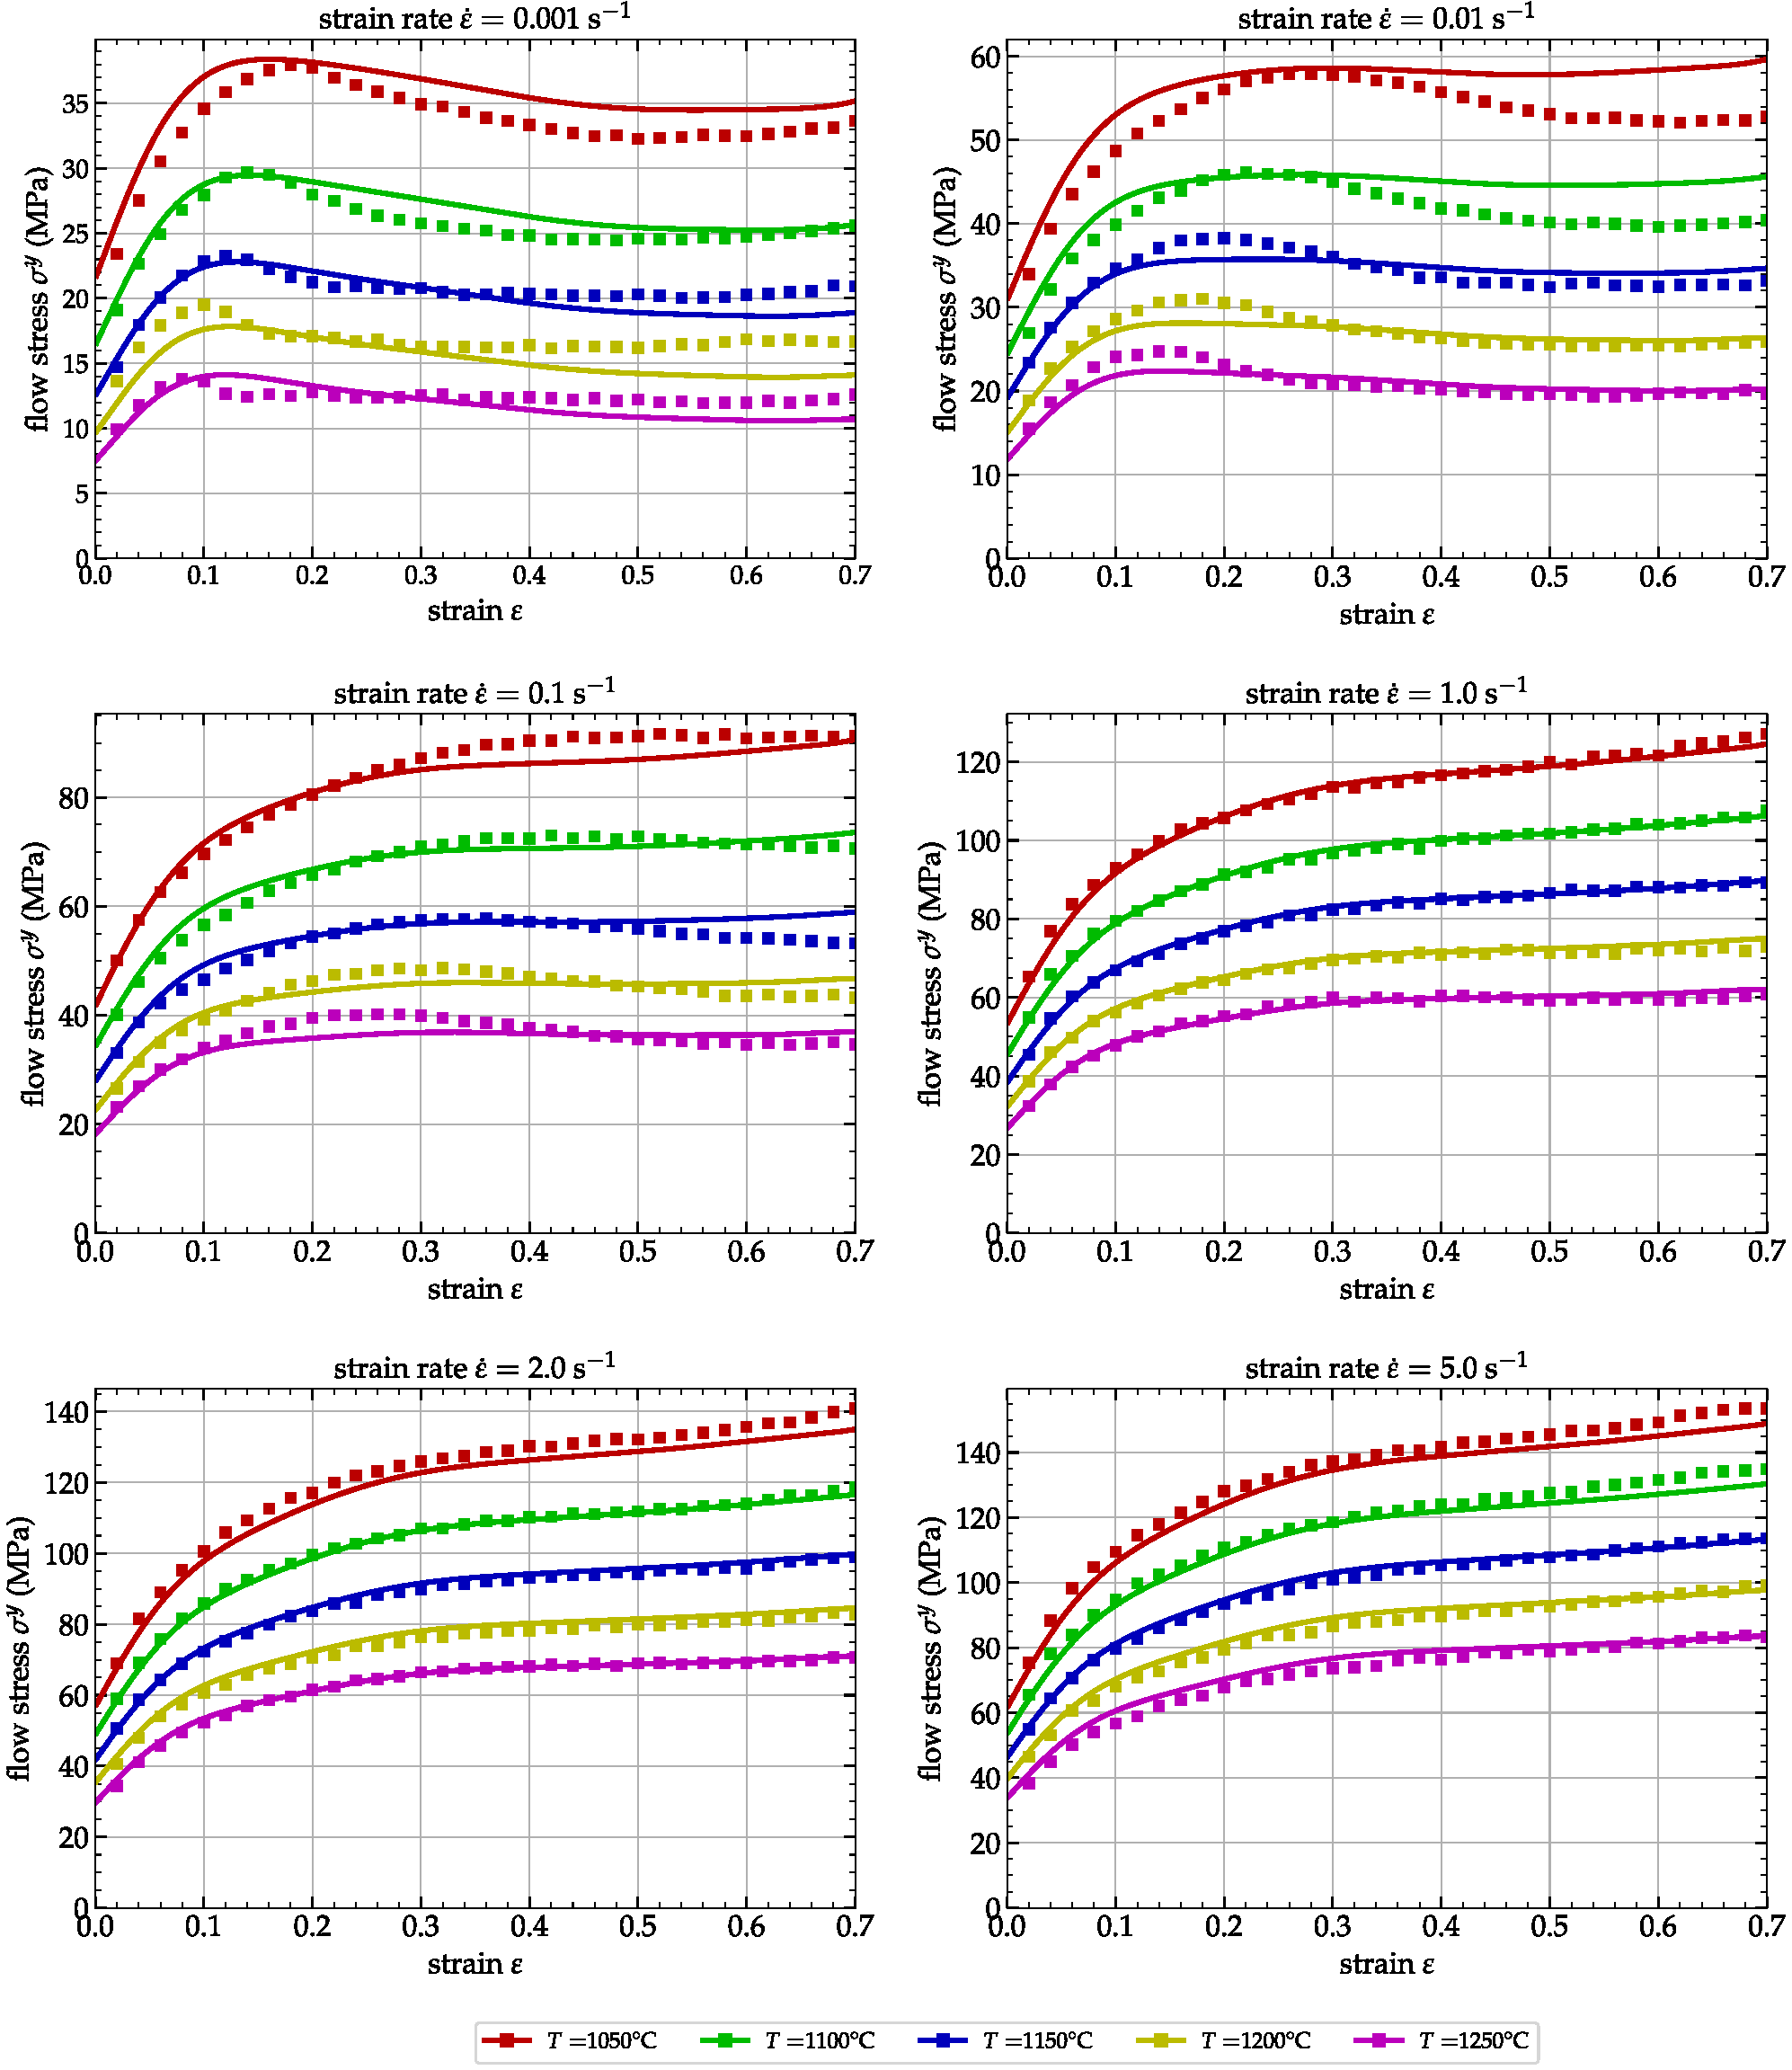
\includegraphics[width=1.02\columnwidth]
{Figures/CompExp-AR-6}
\caption{Comparison between the experimental and predicted flow stresses by AR model}
\label{fig:CompExp-AR-6}
\end{figure}

%-------------------------------------------------------------------------
\subsection{PTM model\label{sec:PTM}}
%--------------------------------------------------------------------------

The PTM model \cite{TizeMha-2022} is a generalized formulation of the MZA model presented in Section \ref{sec:MZA}.
When establishing its formulation, the main shortcomings of the MZA model were taken into account, in order to make the PTM model flexible for any type of material studied because there is no need for a limited number of parameters as in the MZA model.
Its construction is based on the use of polynomial functions as in the AR model.
Thus, the intrinsic functions of the model, of polynomial type, allow to adjust the model according to the degree selected for each of the 4 constituent polynomials, which provides a good fit for each function.
The equation describing the PTM model is therefore given by :
\begin{equation}
\label{eq:PTM-model}
\sigma^y = \left(\sum_{i=0}^{q}{A_i\varepsilon^{p^i}}\right) \exp\left[\left(\sum_{j=0}^{r}{B_j\varepsilon^{p^j}}\right)\left(T-T_0\right) + \left(\sum_{k=0}^{s}\left(\sum_{l=0}^{t}{C_k^l\varepsilon^{p^l}} \right)\left(T-T_0\right)^k \right)\ln\left( \frac{\mdot\varepsilon}{\mdot{\varepsilon}_0}\right)\right]
\end{equation}
where $A_i, B_j, C_k^l$ are the parameters (Table \ref{tab:PTM}) of the model to be identified using the procedure proposed in  \cite{TizeMha-2022}.
Quantities $q$, $r$, $s$ and $t$ define the degree of the polynomials used to describe the behavior of the material.
The larger these quantities are, the more parameters need to be identified for the PTM model.
The determination of the parameters of this model are calculated thanks to the LMFIT Python library \cite{Newville-2016} and for more details about this model  we invite the reader to read our previous work \cite{TizeMha-2022}.
Thus, all the parameters of this model are calculated with $q=5$, $r=5$, $s=1$ and $t=5$.

Comparison of predicted values of the PTM model and experimental values is shown in Figure \ref{fig:CompExp-PTM-6}.
The PTM model is suitable to describe the flow behavior of AISI P20 steel, but for the two strain rates $\mdot\varepsilon=0.01~\ps$ and $\mdot\varepsilon=0.1~\ps$ the prediction in not quite good.
The deviation between the predicted values and the experimental values for other strain rates is relatively good.
For the PTM model, $\AARE=4.79~\%$ and $\RMSE=4.59~\text{MPa}$ this shows an overall worse performance than the AR model.

\begin{table}[h!]
\centering
\caption{Parameters' values of the PTM flow law for the P20 steel}
\begin{tabular}{llll}
\hline
\multicolumn{1}{c}{$A_i$} & \multicolumn{1}{c}{$B_i$} & \multicolumn{1}{c}{$C_0^i$} & \multicolumn{1}{c}{$C_1^i$}\\
\hline
$A_0=16.8529$ & $B_0=-3.5418\times 10^{-3}$ & $C_0^0=0.1608$ & $C_1^0=-1.9037\times 10^{-5}$\\
$A_1=340.6451$ & $B_1=-0.0132$ & $C_0^1=-0.6202$ & $C_1^1=2.67\times 10^{-3}$\\
$A_2=-1.9594\times 10^{3}$ & $B_2=-4.4888\times 10^{-3}$ & $C_0^2=4.9516$ & $C_1^2=-3.5788\times 10^{-3}$\\
$A_3=4.836\times 10^{3}$ & $B_3=0.2218$ & $C_0^3=-13.1694$ & $C_1^3=-0.0222$\\
$A_4=-5.5176\times 10^{3}$ & $B_4=-0.4988$ & $C_0^4=15.25$ & $C_1^4=0.0609$\\
$A_5=2.4058\times 10^{3}$ & $B_5=0.3211$ & $C_0^5=-6.587$ & $C_1^5=-0.0413$\\
\hline
\label{tab:PTM}
\end{tabular}
\end{table}

\begin{figure}[!ht]
\centering
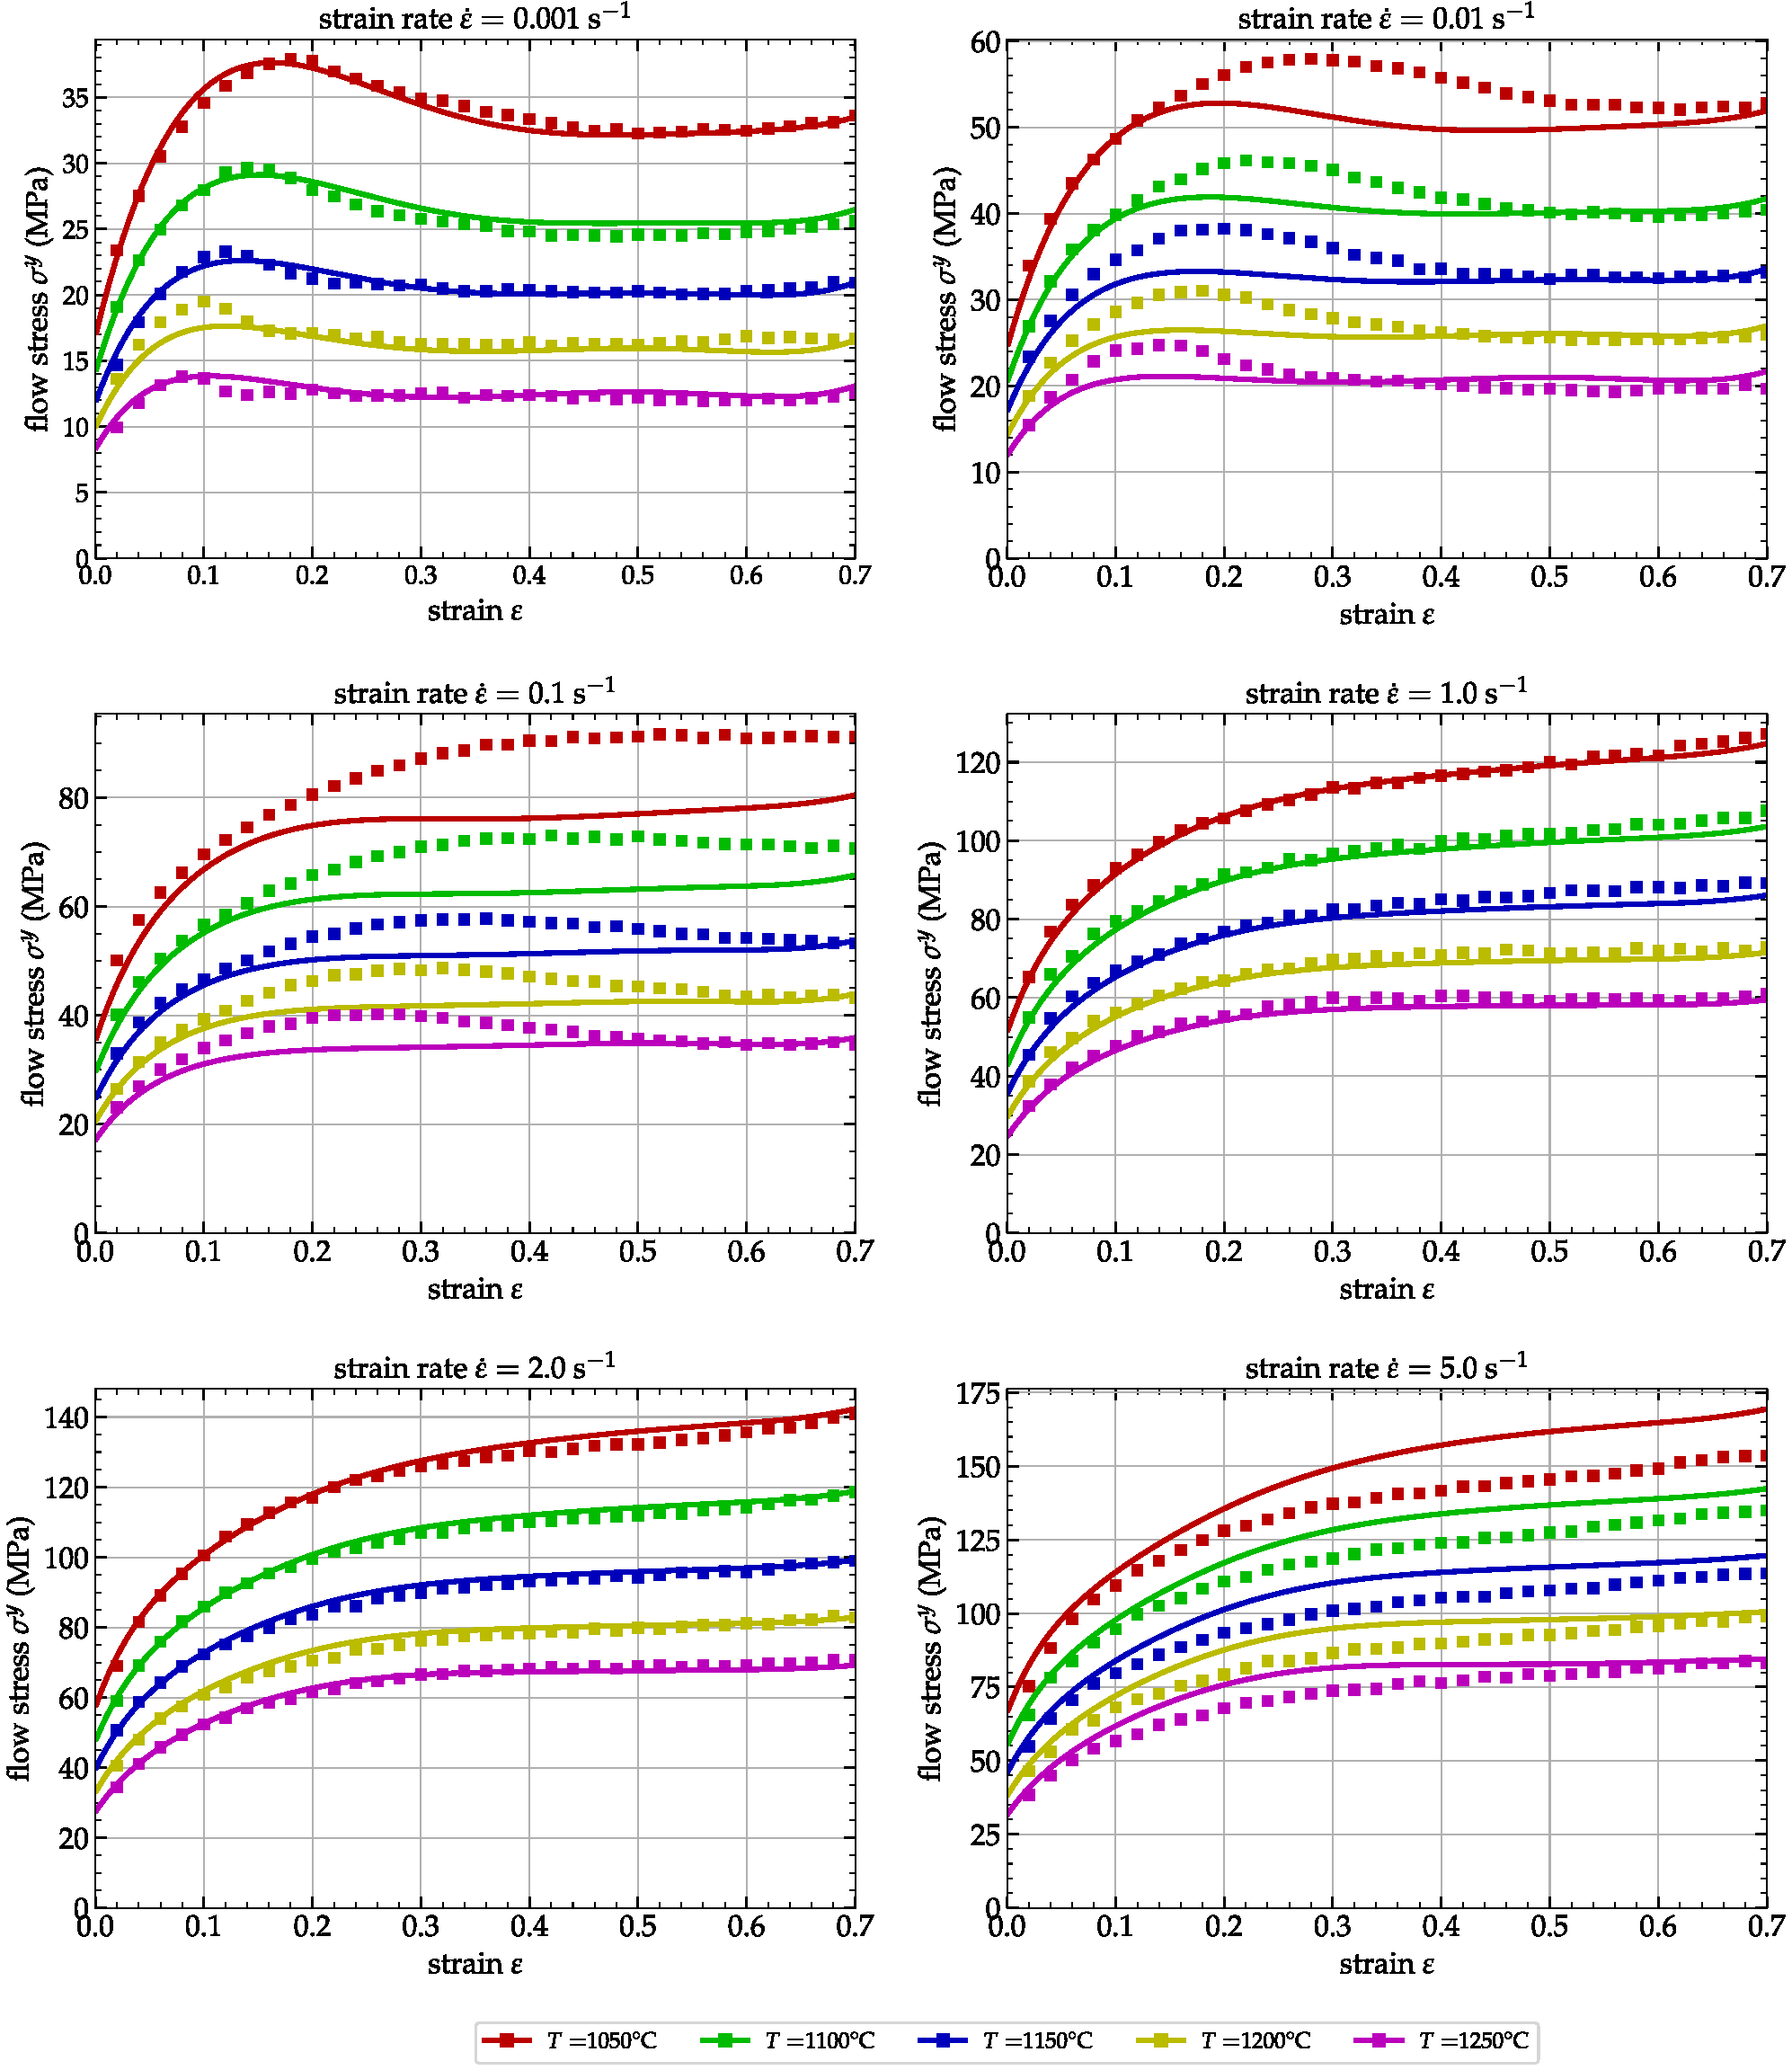
\includegraphics[width=1.02\columnwidth]
{Figures/CompExp-PTM-6}
\caption{Comparison between the experimental and predicted flow stresses by PTM model}
\label{fig:CompExp-PTM-6}
\end{figure}

%-------------------------------------------------------------------------
\subsection{Artificial Neural Network model\label{sec:ANNmodel}}
%--------------------------------------------------------------------------
Because of their predictive capacity and their adaptability, Artificial Neural Networks (ANNs) are more and more widely used today in many scientific fields.
Their operation is based on a learning process during which the principle of minimizing the error between the model's output and the training data allows the adjustment of the model's parameters, as in any machine learning process.

There are generally two uses of neural networks: classification and regression.
The first is the ability to classify data into different groups and for example to distinguish between images of cats and dogs.
The second one corresponds to the capacity of universal approximator of these neural networks, which interests us in this application, and thus to the ability after learning to predict the values of the flow stress $\sigma^y$ according to the input data, as do the analytical models previously identified.
The main difference is that this approximation is not linked to a fixed mathematical formulation (JC, MZA, AR, HS, PTM model), but is only dependent on the data used for training, the number of layers, the number of neurons per layer and the activation functions associated with the neurons of the network.
A feed-forward ANN, as used in our application, contains an input layer, an output layer and a number of hidden layers ($2$ in our case).
Each layer of neurons is connected to the one before it and the one after it by weighted connections.
Thus, all the neurons of the $k$ layer are connected to all the neurons of the ($k-1$) layer as shown in Figure \ref{fig:ANN-2HL}.
\begin{figure}[!ht]
\centering
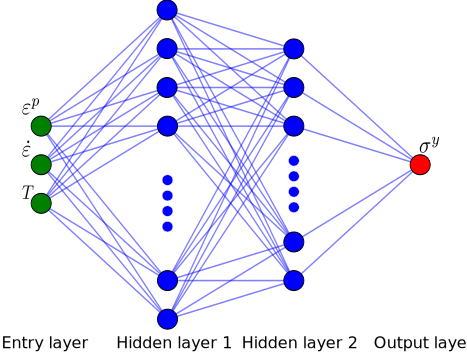
\includegraphics[width=0.7\columnwidth]
{Figures/ANN-scheme-2HL}
\caption{Multi-layer Artificial Neural Network architecture}
\label{fig:ANN-2HL}
\end{figure}

Any hidden layer $k$, containing $n$ neurons, takes a weighted sum of the outputs $\overrightarrow{\hat{y}}$ of the immediately previous layer $(k-1)$, containing $m$ neurons, given by the following equation:
\begin{equation}
y_i\lay{k} = \sum_{j=1}^m w_{ij}\lay{k} \hat{y}_j^{(k-1)}+ b_i\lay{k}\label{eq:ANN1}
\end{equation}
where $y_i\lay{k}$ is the entry of the $i^{th}$ neuron of layer $k$, $\hat{y}_j\lay{k-1}$ is the output of the $j^{th}$ neuron of layer $(k-1)$, $w_{ij}\lay{k}$ is the associated weight parameter between the $i^{th}$ neuron of layer $k$ and the $j^{th}$ neuron of layer $(k-1)$ and $b_i\lay{k}$ is the associated bias of the $i^{th}$ neuron of layer $k$.
Those weights $w_{ij}$ and bias $b_i$, for each layer, are the training parameters of the ANN that we have to adjust during the training procedure described in Pantalé \eal \cite{Pantale-2021}.
For the proposed model, we have selected the ANN2 activation function, so that, each neuron in the hidden layer $k$ provides an output value ${\hat{y}}$ from the input value $y$ of the same neuron defined by Equation (\ref{eq:ANN1}) according to the following equation:
\begin{equation}
\hat{y}=\frac{1}{1 + \e{-y}}\label{eq:ANN2}
\end{equation}
No activation function is used for the output neuron of the ANN.

After some tests of different types of network architecture and in accordance with previous works, a network structure with two hidden layers including $15$ neurons for the first hidden layer and $7$ neurons for the second layer give the best compromise between prediction, learning time and model compactness.
From the global architecture point of view, the input layer is composed of three neurons ($\varepsilon^p$, $\mdot\varepsilon$, $T$) and the output layer is composed of a single neuron corresponding to the $\sigma^y$ flow stress.
This architecture leads to a global model with $180$ parameters to be identified ($60$ for the first layer, $112$ for the second and $8$ for the output).

The Python program used for training the neural network was developed using the specialized Python library Tensorflow \cite{Abadi-2016}.
The Adaptive Moment Estimation (ADAM) optimizer \cite{Kingma-2015} was used for the training phase.
The training data are those from the tests presented in section \ref{sec:ComTestResults} and composed of $21000$ quadruplets of ($\varepsilon^p$, $\mdot\varepsilon$, $T$, $\sigma^y$) values.
The learning is performed on the basis of $5000$ epochs of the experimental data set.
Fourty minutes of training on a Dell XPS-13 7390 laptop running Ubuntu 22.04 LTS 64 bits with 16 GiB of Ram and an Intel 4-core i7-10510U processor allow obtaining the converged parameters of the ANN model.
Figure \ref{fig:ANN-6-conv} show the evolution of the training error defined by the $\log_{10}$ of the Root Mean Square Error during the training phase.
\begin{figure}[!ht]
\centering
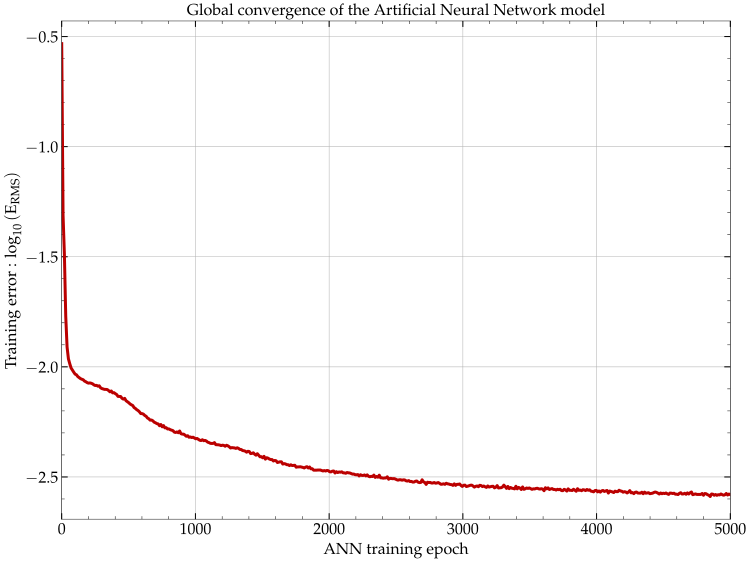
\includegraphics[width=0.7\columnwidth]
{Figures/Conv-ANN-6}
\caption{Convergence of the ANN model during the training phase.}
\label{fig:ANN-6-conv}
\end{figure}
As we can see on this figure, after $5000$ epoch, we can consider that we have reached a stationary state of the model learning and that it is useless to continue the learning phase.

Once the learning phase is over, the trained model can be used to predict the behavior of the AISI P20 alloy as a function of the input data in the same way as is done with the analytical models.
One can either use the model directly by providing it with new input data, or retrieve the $180$ parameters identified during the training and inject them into a mathematical model based on Equations (\ref{eq:ANN1}) and (\ref{eq:ANN2}) which can be implemented in any language (\eg in FORTRAN for use on the Abaqus Explicit FEM code) as proposed in Pantalé \eal \cite{Pantale-2021}.
For reasons of compactness, the parameters of the ANN model and the complete procedure to compute the flow stress $\sigma^y$ from the input data are provided in the Appendix.

As for the analytical models presented previously, Figure \ref{fig:CompExp-3-15-7-1-sigmoid} shows a comparison between the flow stresses predicted by the ANN model and the data measured during the hot compression test.
\begin{figure}[!ht]
\centering
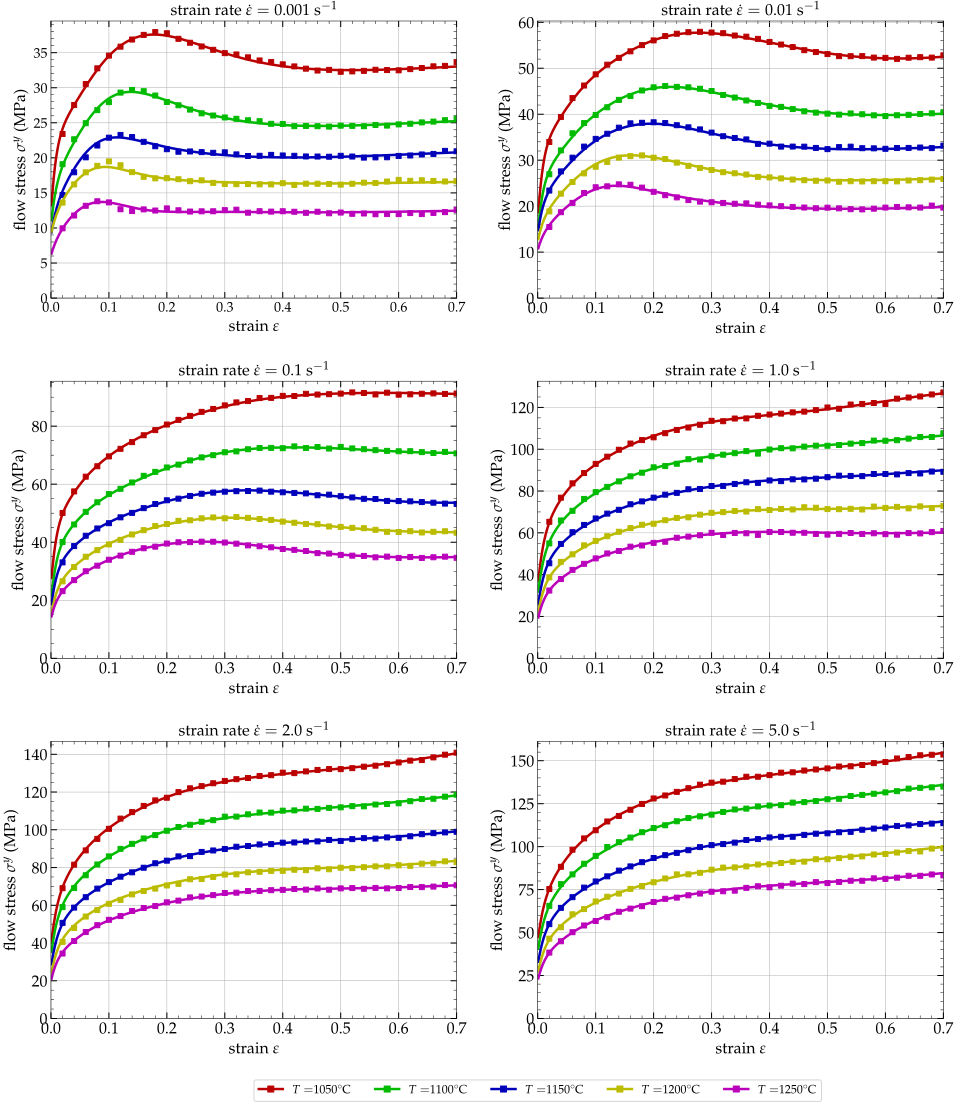
\includegraphics[width=1\columnwidth]
{Figures/CompExp-3-15-7-1-sigmoid}
\caption{Comparison between the experimental and predicted flow stresses by the 3-15-7-1-sigmoid ANN model}
\label{fig:CompExp-3-15-7-1-sigmoid}
\end{figure}
The correlation between the experimental data and the ANN prediction is very good over the entire range of data and the predicted data can track the hardening and softening regions of the hot deformed material well.
For the ANN model, $\AARE=0.62~\%$ and $\RMSE=0.38~\text{MPa}$ which is excellent.
This model can be used to simulate the hot deformation of this type of alloy with much greater fidelity to the actual material behavior than the analytical models presented previously.

%-------------------------------------------------------------------------
\subsection{Comparison of analytical and ANN models\label{sec:Comparison}}
%--------------------------------------------------------------------------

A summary of the coefficients for evaluating the high-temperature flow stress prediction capability of the AISI P20 alloy for all models presented in this work is reported in Table \ref{tab:Errors}.
\begin{table}[h!]
\centering
\caption{Accuracy coefficients for all the analyzed models.}
\begin{tabular}{lcccccc}
\hline
Coefficients & JC & MZA & HS & Arhenius & PTM & ANN\\
\hline
$\AARE(\%)$ & $14.05$ & $21.20$ & $7.75$ & $3.56$ & $4.79$ & $0.62$\\
$\RMSE(\text{MPa})$ & $12.00$ & $19.57$ & $3.80$ & $2.18$ & $4.59$ & $0.38$\\
\hline
\label{tab:Errors}
\end{tabular}
\end{table}
From this table, we can see that the ANN model has a much better predictive capacity than all the analytical models presented previously.The values of $\AARE$ and $\RMSE$ are globally $6$ times lower than the best of the analytical models, \ie the Arrhenius model, quoted as reference in the context of hot forming of alloys \cite{Liang-2022}.

The ANN, Arrhenius and PTM models are the only models that take into account the softening with the deformation of AISI P20 at low strain rate, unlike the other three models that only present an increase of the flow stress with the strain, whatever the strain rate and temperature, hence their poor performance in predicting the behavior of this material and more particularly at low strain rates.
The parameters reported in Table \ref{tab:Errors}, the correlations visible in Figures \ref{fig:CompExp-JC-6} to \ref{fig:CompExp-3-15-7-1-sigmoid} allow us to conclude here that the ANN model is the most efficient of all the models presented to describe the behavior of the AISI P20 alloy for high temperature deformation applications.

%-------------------------------------------------------------------------
\section{Interpolation and extrapolation capability of phenomenological and ANN models \label{sec:inExtrapolation}}
%--------------------------------------------------------------------------
In this section we wish to test the performance of each identified model data interpolating and extrapolating data.
Indeed, out of the $6$ strain rates used, one strain rate is voluntarily removed (while keeping the same values of strains and temperatures used for the development of the phenomenological and ANN models) so that it is inside or outside the other $5$ strain rates.
For the strain rate which is between the minimum and the maximum of the $5$ other strain rates, we will thus test the capacity of each model to interpolate the data and for the one which is out of the $5$ other strain rates, the extrapolation capacity of the model is therefore validated.
The validation procedure is as follows: $5$ strain rates are used to re-identify each model and once identified, it is used to predict the flow stress for the strain rate chosen for both interpolation and extrapolation.
Validation is done with real data.
The following subsections will highlight this procedure.
\subsection{Interpolation validation}
For the validation of the interpolation, the chosen strain rate is $\mdot\varepsilon = 1.0\ \ps$ and those used for identification (training for ANN) are $\mdot\varepsilon = 0.001\ \ps$ , $\mdot\varepsilon = 0.01\ \ps$ , $\mdot\varepsilon = 0.1\ \ps$, $\mdot\varepsilon = 2.0\ \ps$  and $\mdot\varepsilon = 5.0\ \ps$.
The Figure \ref{fig:IntComp} shows the comparison between the predictions of the analytical and ANN models and the experiment.
It appears from these Figures that all models have relatively good predictions but the ANN model remains the best because the value of its $\AARE$ is $1.4\%$ while it is between $2.33\%$ and $6.13\%$ for the analytical models.
This further shows the performance of the ANN model compared to the analytical models.
All these results are summarized in Table \ref{tab:IntVal}.
\begin{figure}[!ht]
\centering
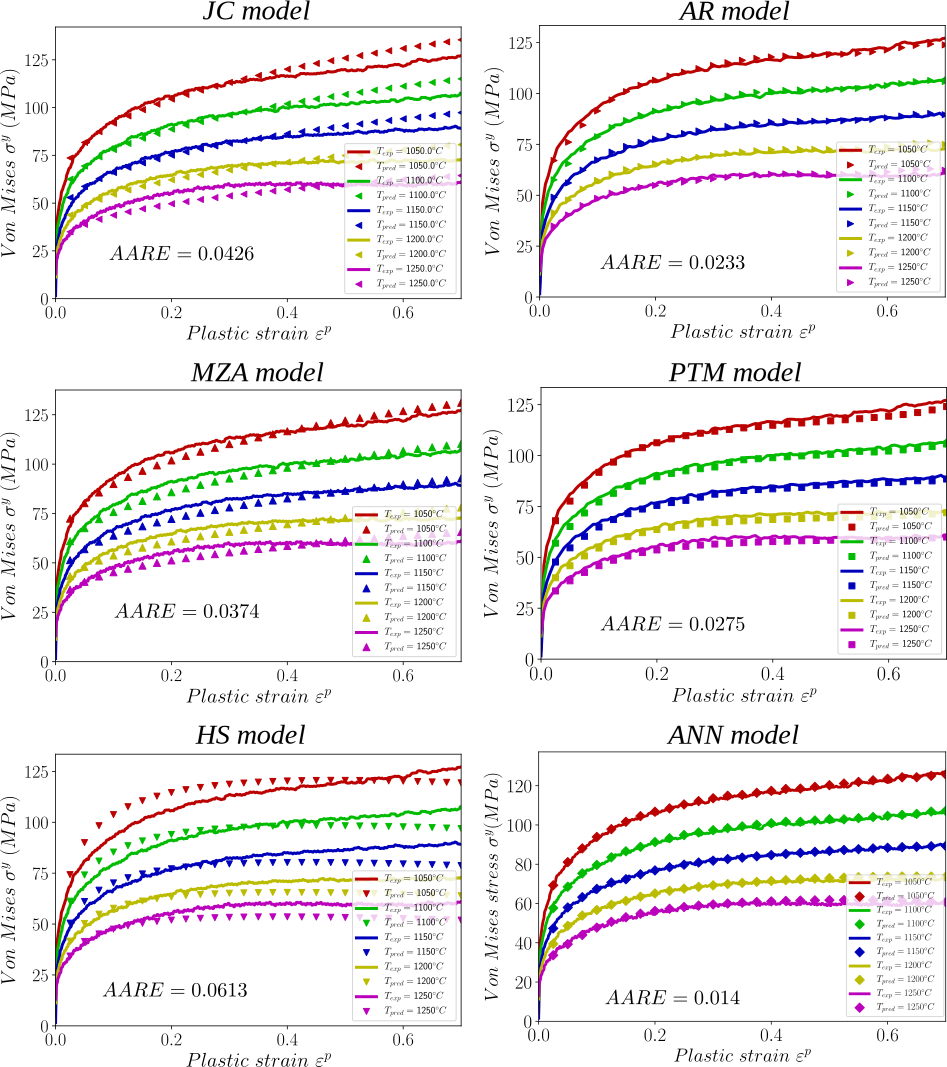
\includegraphics[width=1.02\columnwidth]
{Figures/inCombinaison}
\caption{Comparison between the experimental and predicted flow stresses by ANN model for interpolation estimation}
\label{fig:IntComp}
\end{figure}
\begin{table}[h!]
\centering{}
\caption{Accuracy coefficients of interpolation}
\begin{tabular}{lcccccc}
\hline
&		&		&         &             &		   &	\\
Coefficients&JC  & MZA  &HS  & Arhenius      & PTM  &ANN \\
&				&				&         &             &	&\\
\hline
$R(\%)$&$99.0590$&$99.0821$&$97.6008$&$99.8417$& $99.8760$&$99.9439$  \\
$\AARE(\%)$&$4.2686$&$3.7440$&$6.1391$&$2.3321$&$2.7590$&$1.4018$   \\
$\RMSE(\text{MPa})$&$4.1923$&$3.1856$&$82.6956$&$2.29891$&$2.4632$&$1.0228$ \\
\hline
\label{tab:IntVal}
\end{tabular}
\end{table}
\subsection{Extrapolation validation}
For the validation of the extrapolation, the chosen strain rate is $\mdot\varepsilon = 5.0\ \ps$ and those used for identification (training for ANN) are $\mdot\varepsilon = 0.001\ \ps$ , $\mdot\varepsilon = 0.01\ \ps$ , $\mdot\varepsilon = 0.1\ \ps$, $\mdot\varepsilon = 1.0\ \ps$  and $\mdot\varepsilon = 2.0\ \ps$.
Figure \ref{fig:ExtComp} shows the comparison between the predictions  and the experimental.
Unlike interpolation, the predictions of the analytical models are not very good because the errors are between $3.2\%$ and $12.99\%$ while that of the ANN model is $1.74\%$.
Again, the ANN model shows its ability to extrapolate data.
This makes it possible to say that the ANN model remains the best tool to characterize the behavior of a material subjected to certain deformation conditions.
It can also be noted that the Arhenius and the PTM models still have some ability to extrapolate because their $\AARE$ are respectively $ 3.2 \% $ and $ 3.8 \%$; which are acceptable.
\begin{table}[h!]
\centering{}
\caption{Accuracy coefficients of extrapolation}
\begin{tabular}{lcccccc}
\hline
&		&		&         &             &		   &	\\
Coefficients&JC  & MZA  &HS  & Arhenius      & PTM  &ANN \\
&				&				&         &             &	&\\
\hline
$R(\%)$&$99.2920$&$99.4879$&$93.9429$&$99.6870$& $99.7582$&$99.8047$\\
$\AARE(\%)$&$4.8988$&$3.4506$&$12.9939$&$3.2008$&$3.8845$&$1.7433$\\
$RMSE(\text{MPa})$&$5.0943$&$4.3048$&$116.517$&$3.7035$&$4.3915$&$1.2513$ \\
\hline
\label{tab:ExtVal}
\end{tabular}
\end{table}
\begin{figure}[!ht]
\centering
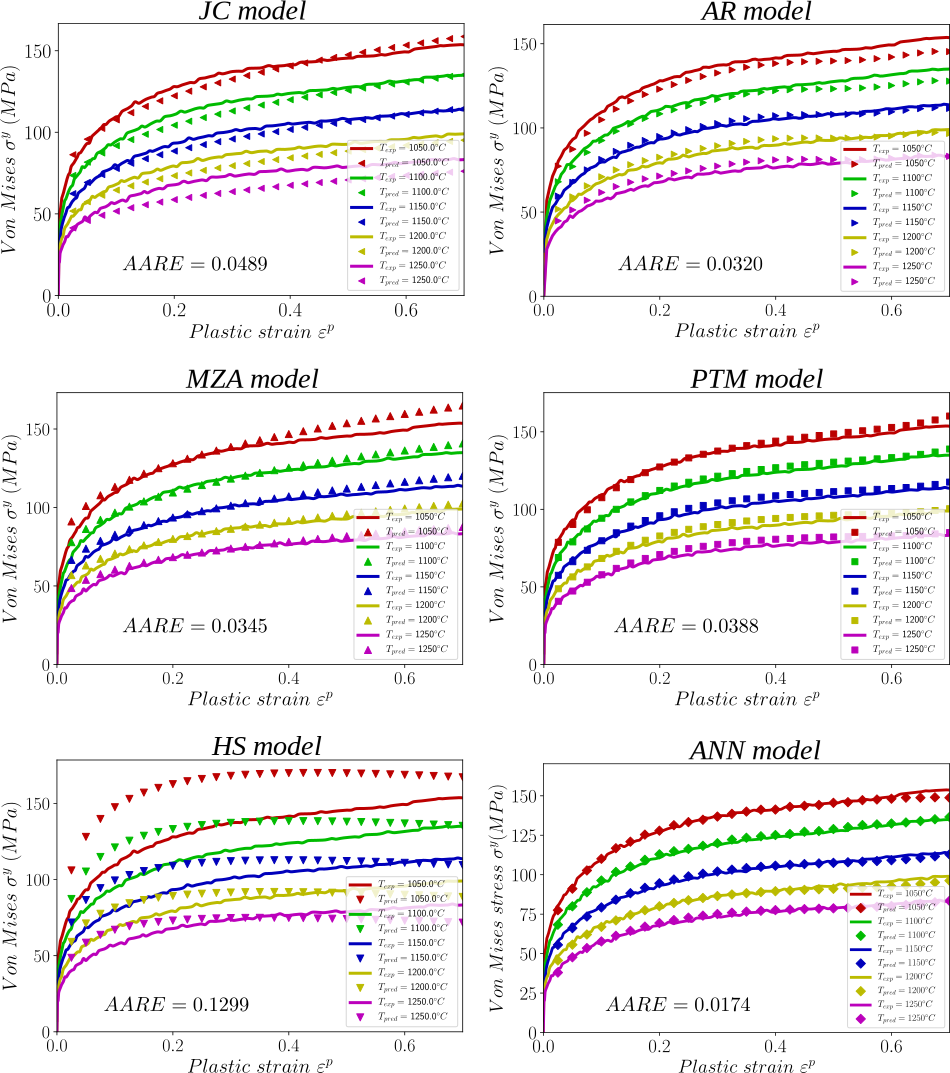
\includegraphics[width=0.91\columnwidth]
{Figures/exCombinaison}
\caption{Comparison between the experimental and predicted flow stresses by ANN model for extrapolation estimation}
\label{fig:ExtComp}
\end{figure}

%---------------------------------------------------------------------
\section{Conclusion \label{sec:Conclusion}}
Experiments were conducted on modified AISI P20 carbon alloy to study the applicability and predictive accuracy of five analytical models and one neural network model over a range of temperatures ($1050\celsius$ - $1250\celsius$, strains ($0.025$ - $0.7$), strain rates ($0.001\ \ps$ - $5\ \ps$) and the following conclusions were drawn.
\begin{enumerate}
\item The flow stress increases with decreasing temperature and increasing strain rate due to the competitive occurrence of dynamic softening and strain hardening mechanisms.
The degree of DRX was discussed through the difference between the maximum and permanent stress, as well as the evolution of the microstructure which shows a partially complete DRX.
At high strain rates it is difficult to visualise the DRX phenomenon on the flow curves due to the strain rate sensitivity of this phenomenon.
A further study will focus on deep analysis of the microstructure of this steel alloy and its impact on mechanical properties.
\item Five analytical models have been identified on this alloy and a model based on neural networks.
Among the analytical models, the JC, HS and MZA models proved inappropriate for analysing the behavior of this material whereas the PTM and AR models showed their capacity since they have a relatively acceptable error ($ 3.2 \% $ and $ 3.8 \%$).
As for the ANN model, it is largely reliable that the analytical models to predict the competitiveness of AISI P20.
Therefore it may be advisable to use the ANN model when conducting a study involving this alloy under these experimental conditions.
\item To test the performance of each model, a study is carried out to evaluate the interpolation and extrapolation capacity of the developed models.
For the interpolation framework, all models have a good correlation with the experiment except the HS model but the ANN model shows a better correlation.
For extrapolation of the data, the analytical models do not show good predictive capacity compared to the ANN model which still shows good extrapolation capacity.
This further confirms what was demonstrated during his identification.
\item As perspectives of this work, we will develop also an ANN model to characterize the microstructure in terms of DRX and phase formation such as fearrite, bainite and martensite as an example.
This ANN model can therefore be compared to the most commonly used classical models such as the JMAK model.
Therfore, this ANN model  will be implemented in FEM softwares such as Abaqus, Forge in order to validate it by doing a simulation.
\end{enumerate}

\bibliographystyle{elsarticle-num}
\bibliography{Bibliography}

\section*{Appendix\label{sec:Appendix}}
In order to complete this paper, we report here after the computing process and the $180$ coefficients of the Artificial Neural Network ANN-3-15-7-1-sigmoid model used in Section \ref{sec:ANNmodel}. In order to use this model we describe here after the procedure to compute the flow stress $\sigma^y$ from the input variables $\varepsilon^p$, $\mdot\varepsilon$ and $T$. This process can be decomposed in $3$ phases:
\begin{itemize}
\item We first have to normalize the input values of the ANN $x_i$ within the range $[0,1]$ to avoid ill-conditioned system as presented by many other authors in the literature \cite{Lin-2008-ANN, Lu-2011-ANN}.
Therefore, the three components of the input are obtained from the plastic strain $\varepsilon^p$, the plastic strain rate $\mdot{\varepsilon}^p$ and the temperature $T$ using the following expressions:
\begin{equation}
\begin{cases}
x_1 = \frac{\varepsilon^p - [\varepsilon^p]_{min}}{[\varepsilon^p]_{max} - [\varepsilon^p]_{min}}\\
x_2 = \frac{\ln(\mdot{\varepsilon}/\mdot{\varepsilon_0})-[\ln(\mdot{\varepsilon}/\mdot{\varepsilon_0})]_{min}}{[\ln(\mdot{\varepsilon}/\mdot{\varepsilon_0})]_{max}-[\ln(\mdot{\varepsilon}/\mdot{\varepsilon_0})]_{min}}\label{eq:CR1}\\
x_3 = \frac{T-[T]_{min}}{[T]_{max}-[T]_{min}}
\end{cases}
\end{equation}
where $[~]_{min}$ and $[~]_{max}$  are the boundaries of the range of the corresponding field: $\varepsilon^p\!\in\!\left[0.0,0.7\right]$, $\mdot{\varepsilon}\!\in\!\left[0.001,5.0\right]$, $T\!\in\!\left[1050,1250\right]$ and $\sigma\!\in\!\left[1.311,153.739\right]$. The reference strain rate is $\mdot{\varepsilon_0} = 0.001$.
\item Then we compute the output $s$ of the ANN from the input vector $\overrightarrow{x}$ using the three following equations.
\begin{equation}
\overrightarrow{y}_1 = \left[1 + \exp{\left(- \w_1 \dotp \overrightarrow{x}- \overrightarrow{b}_1\right)}\right]^{-1}
\end{equation}
\begin{equation}
\overrightarrow{y}_2 = \left[1 + \exp{\left(- \w_2 \dotp \overrightarrow{y}_1- \overrightarrow{b}_2\right)}\right]^{-1}
\end{equation}
\begin{equation}
s = \overrightarrow{w}^T \dotp \overrightarrow{y}_2 + b
\end{equation}
\item Finally, the flow stress $\sigma^y$ can be obtained from the output $s$ of the ANN using the following equation:
\begin{equation}
\sigma^y =  \left([\sigma]_{max}-[\sigma]_{min}\right)s + [\sigma]_{min} \label{eq:CR2}
\end{equation}
\end{itemize}

Conforming to the computing process proposed by Equations (\ref{eq:CR1}-\ref{eq:CR2}), we report hereafter the $180$ coefficients of the ANN-3-15-7-1-sigmoid model used in Section \ref{sec:ANNmodel}.

\begin{equation*}
\w_1^T = \left[
\begin{array}{rrr}
2.2206 & -3.7555 & -6.7246\\ 
-4.8598 & 5.7431 & -5.8538\\ 
2.3099 & 3.3325 & -5.1795\\ 
2.0475 & 0.8006 & -1.4259\\ 
8.8358 & -6.0362 & 0.8226\\ 
-1.2613 & -0.9274 & -2.3725\\ 
-0.3561 & 6.5032 & -10.7573\\ 
-11.7226 & -2.0455 & 1.2248\\ 
3.1066 & 26.5580 & 18.6540\\ 
-0.5150 & -5.6922 & 1.0104\\ 
-6.4755 & 8.4888 & -2.4459\\ 
-1.8791 & -0.5380 & 2.2295\\ 
-6.0206 & 1.2776 & 0.2169\\ 
0.2619 & -4.7974 & -1.1282\\ 
-27.1456 & -0.5327 & -0.5303\\ 
\end{array}\right]
\end{equation*}
\begin{equation*}
\overrightarrow{b}_1 = \left[
\begin{array}{r}
5.9164\\ 
-1.9074\\ 
-2.6837\\ 
-1.0954\\ 
-0.9509\\ 
3.1682\\ 
-4.3964\\ 
0.6343\\ 
-5.0676\\ 
2.0228\\ 
1.1267\\ 
-0.9671\\ 
-0.6263\\ 
2.3110\\ 
-0.3037\\ 
\end{array}\right]
\end{equation*}
\begin{equation*}
\w_2 = \left[
\begin{array}{rrrrrrr}
-0.5783 & 1.2724 & 0.5747 & 0.6449 & -4.2203 & -0.2380 & 0.2591\\ 
-0.4852 & 5.2807 & 0.8888 & -8.2324 & -2.0075 & -0.6474 & -1.0787\\ 
4.4499 & -0.0137 & 0.1657 & 0.3198 & 4.9765 & -1.2503 & 0.8219\\ 
1.7571 & 0.7730 & 0.0208 & -1.3316 & -0.8945 & -0.7284 & -0.1831\\ 
-1.0866 & 0.1330 & -0.8615 & -0.1283 & 0.2218 & -0.1772 & -2.7458\\ 
-0.3925 & 1.3994 & 0.0630 & -1.8397 & -1.1047 & -1.9839 & 0.5767\\ 
-0.2121 & 0.9977 & 1.2028 & -9.6525 & 0.5520 & 0.1062 & -0.0409\\ 
-1.1518 & -1.6402 & -4.1501 & -1.0759 & 0.4749 & -2.8350 & 0.9225\\ 
-1.1453 & -0.2173 & -0.1382 & 0.8264 & -0.5125 & 0.1882 & -0.8654\\ 
-4.3301 & -0.3711 & -7.4305 & 3.5926 & -9.6217 & -1.2375 & 1.6171\\ 
2.3907 & -1.0085 & -0.8828 & -1.1891 & 0.9947 & 1.1178 & -1.0953\\ 
-1.5955 & 1.6313 & 0.4916 & 0.1906 & -1.9216 & -1.4140 & 1.3827\\ 
-1.6985 & 1.4277 & -3.4462 & -8.3777 & -1.2132 & -1.2158 & 2.8512\\ 
-1.9954 & -2.0159 & -8.3455 & -0.5205 & 0.2942 & -1.3337 & 0.2026\\ 
4.3040 & -0.7164 & -1.0859 & 3.4294 & -23.8003 & 12.5859 & 7.3721\\ 
\end{array}\right]
\end{equation*}
\begin{equation*}
\overrightarrow{b}_2 = \left[
\begin{array}{r}
0.7534\\ 
0.9473\\ 
0.6055\\ 
-0.7793\\ 
-1.0305\\ 
-1.5779\\ 
-0.1471\\ 
\end{array}\right]
\end{equation*}
\begin{equation*}
\overrightarrow{w}_3 = \left[
\begin{array}{r}
0.1920\\ 
0.3406\\ 
0.3839\\ 
-0.2880\\ 
1.2047\\ 
-1.4126\\ 
-0.2215\\ 
\end{array}\right]
\end{equation*}
\begin{equation*}
b_3 = 0.1178 
\end{equation*}

\end{document}


